%
%
%
%
%
\chapter{Semi-structured Mesh Generator for Turbomachinery Blades}
 \label{mesh.chap}
\heada{Semi-structured Mesh Generator}
\setcounter{footnote}{0}
%
\newcommand{\fdx}[1]{\frac{\partial }{\partial {#1} }}
\newcommand{\fpa}[3]{\frac{\partial {\mathbf{#1}}_{#2} }{\partial {#3} }}
\newcommand{\spd}[2]{\frac{\partial^2 {#1} }{\partial {#2}^2 }}
\newcommand{\sxd}[3]{\frac{\partial^2 {#1} }{\partial {#2} \partial {#3} }}
%
%
 This chapter describes the development of a novel
 mesh generator for the flow analysis of turbomachinery blades. The
 proposed method uses a combination of structured and unstructured meshes,
 the former in the
 radial direction and the latter in the axial and tangential
 directions in order to exploit the fact that blade-like structures
 are not strongly 3D since the radial variation
 is usually small. The proposed semi-structured mesh formulation was found to
 have a number of advantages over its structured counterparts.
 There is a significant improvement
 in the smoothness of the grid-spacing and in capturing
 particular aspects of the blade passage geometry. It was also found that
 the leading- and trailing-edge regions could be  discretised without generating
 superfluous points in the far field and that further refinements of the mesh
 to capture wake and shock effects were relatively easy to implement.
%
%
%%%%%%%%%%%%%%%%%%%%%%%%%%%%%%%%%%%%%%%%
%%%%     INTRODUCTION
%%%%%%%%%%%%%%%%%%%%%%%%%%%%%%%%%%%%%%%%
%
%
\section{Introduction}
\headb{Semi-structured Mesh Generator}{Introduction}
%
 It is well known that the grid structure must be selected carefully
 in order to achieve an accurate resolution of complex flow fields
 typical of axial-flow turbomachines.
 The minimization of skewness and the optimization of smoothness
 generally result in a faster convergence as well as less solution dependence
 on the grid density, therefore reducing
 computational cost both in terms of memory and CPU time.
 As a consequence, the grid generation procedure should be considered
 an integral part of the numerical method.

 When performing a numerical simulation of turbulent-viscous flow in turbomachinery
 passage, the following aspects are of importance: i)
 accurate leading- and trailing-edge flow descriptions, ii) wake resolution,
 iii) proper gridding in the throat area where most of the shock
 is expected to occur, and iv) imposition of periodicity.

 Historically, mesh generation techniques for turbomachinery blades use
 structured hexahedral representations, the most commonly
 used ones being H-type, C-type, and O-type. These meshes are obtained either
 by using an algebraic approach (Kallinderis \& Ward \citeyearNP{Kallinderis:1})
 or by solving a system of elliptic
 partial differential equations (Thompson et al. \citeyearNP{Ellipt1},
 Steger \& Sorenson \citeyearNP{Ellipt2}, Brackbill \& Saltzman
 \citeyearNP{Ellipt3}) or by solving hyperbolic partial differential equations
 (Steger \& Chaussee \citeyearNP{Ellipt4}).
 H-type meshes have been by far the most common choice in turbomachinery
 applications as they are very easy to generate, the imposition of
 periodicity is straightforward and the mesh density before, inside,
 and after the blade passage can be easily controlled. However,
 the leading- and trailing-edge descriptions are poor and a large
 amount of superfluous points is generated in the region between
 the inflow and the leading-edge. A classical H-mesh for a transonic blade
 is shown in Fig. \ref{Hmesh.fig}.
%
\begin{figure}[ht]
  \centerline{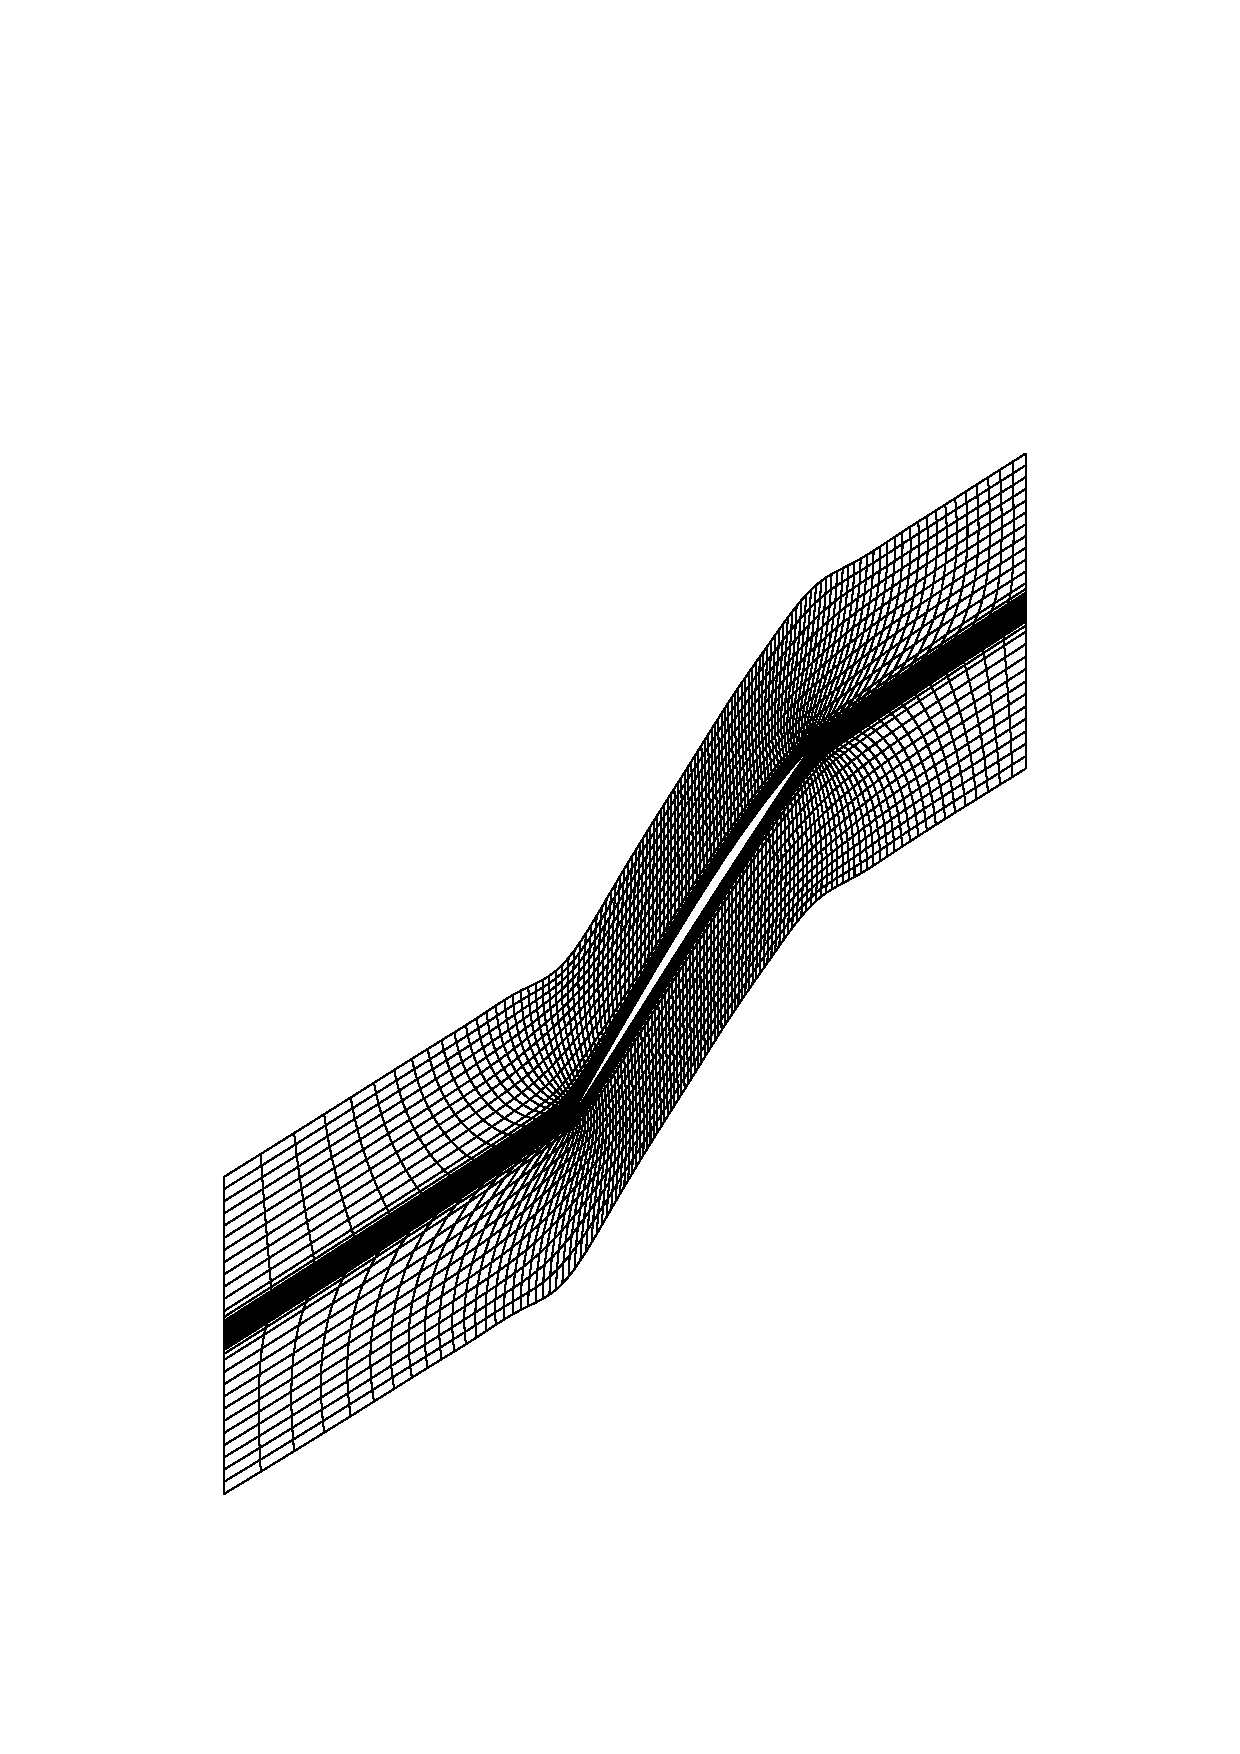
\includegraphics[width=50mm,clip=t]{CHAP_MESH/FIGURE/Hmesh.pdf}}
 \caption{Typical structured H-mesh for a fan blade geometry}
 \label{Hmesh.fig}
\end{figure}
%
 O-type grids are not very effective in capturing the wake and their
 quality outside the passage is very poor. This can smear
 the bow shock away from the leading edge of a transonic compressor
 or the outgoing shock of a transonic turbine blade.
 On the other hand, C-type meshes can capture the wake structure if
 they are carefully generated but their quality in the region between
 the inflow and the leading-edge is not suitable to resolve bow shock
 accurately.

 A different approach is to use unstructured triangular meshes
 for 2D turbomachinery calculations. Fully unstructured grids
 offer good flexibility and most of the flow features can be captured with
 good accuracy via mesh refinement.
 3D unstructured meshes are widely used in external aerodynamics but
 they have rarely been applied to turbomachinery cases.
 The main difficulty associated with such meshes is their isotropic
 nature. The very fact that tetrahedral unstructured meshes do not exhibit
 any preferred direction is what makes them ideal for discretising arbitrarily
 complex configurations. In fact most of the unstructured mesh generation
 techniques rely on this property.
 However, when a configuration with a preferred direction, such as a
 turbomachinery blade, is to be discretised,
 and different resolutions  are desired in the various directions, unstructured mesh
 generation techniques are known to experience great difficulties in
 meeting such requirements. Turbomachine blades require high resolution near
 their leading and trailing edges and radial spacing can be relatively coarse.
 When using an isotropic unstructured mesh,
 the high leading and trailing edge resolution requirements also result in
 a high radial resolution in these areas, a feature greatly increases the
 number of grid points. Such a degree of radial resolution is superfluous,
 since the radial gradients are known to be relatively small for turbomachinery
 blade flows.
 Similar difficulties occur in the boundary layer regions near a wall for
 high Reynolds number viscous flows, where the normal gradients are several
 orders of magnitude grater than the stream-wise gradients.
 To illustrate the unsuitability of unstructured meshes
 for such applications, a fully unstructured mesh was created for fan blade
 geometry using an advancing front technique (Morgan et al. \citeyearNP{Peiro:1}),
 the suction side being shown in Fig. \ref{unstruct.fig}.
%
\begin{figure}[ht]
   \centerline{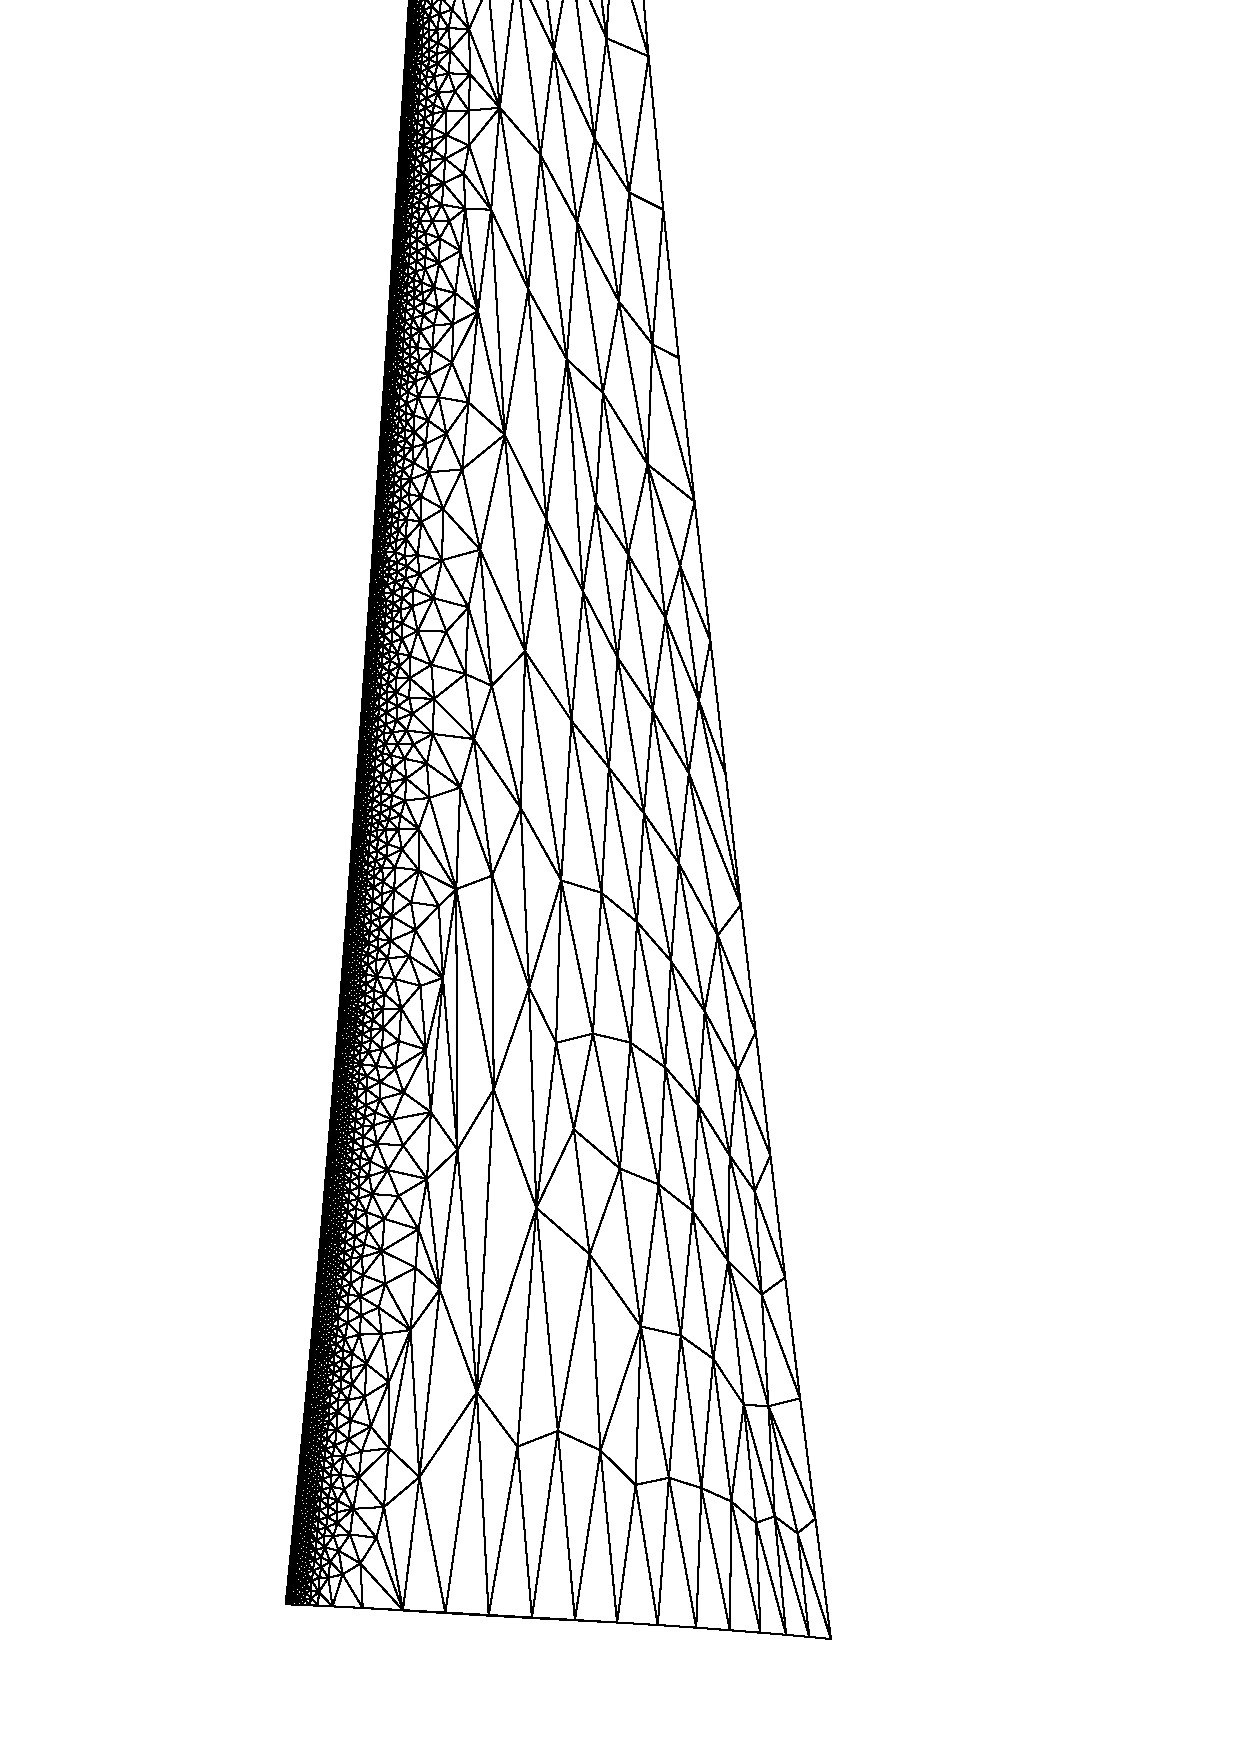
\includegraphics[width=30mm,clip=t]{CHAP_MESH/FIGURE/unstruct.pdf}}
   \caption{Fully unstructured mesh on suction surface}
   \label{unstruct.fig}
\end{figure}
%
 It is clearly seen that a large number of points are needed in the leading
 edge area in order to satisfy the resolution
 requirements, a feature which creates an unacceptably high overhead
 in the total number of points. It should also be noted that, for
 this particular geometry, the generation of an efficient viscous mesh
 will be very difficult using a totally unstructured grid because of the
 boundary layer considerations.

 The considerations above lead to the use of semi-structured meshes
 for turbomachinery blades. The aim of this chapter is to present a
 novel approach for discretising turbomachinery blades by using a combination
 of structured and unstructured meshes, the former in the radial direction
 and the latter in the axial and tangential directions.
 The basic idea relies on the fact that blade-like structures
 are not strongly 3D since the radial variation
 is usually small.
 It is therefore possible to start with a structured
 and body-fitted 2D O-grid around a given aerofoil section
 to resolve the boundary layer.
 This core mesh is then extended in an unstructured
 fashion up to the far-field boundaries,
 the triangulation being performed using an advancing
 front technique (Morgan et al. \citeyearNP{Peiro:1},
 Mavriplis \citeyearNP{Mavriplis:2}).
 Once this 2D grid is generated, it is projected to the remaining radial
 sections via quasi-conformal mapping techniques.
 When all such radial sections are formed, a 3D
 prismatic grid is obtained by simply connecting the corresponding
 points of different layers. In this way, hexahedral
 elements are generated in the viscous region and
 triangular prisms in the rest of the solution
 domain. Again, such an approach presents a distinct advantage over
 totally unstructured grids which are usually confined to tetrahedral
 elements only, though this limitation is usually a consequence of the
 unavailability of general viscous mesh generators.
%
%%%%%%%%%%%%%%%%%%%%%%%%%%%%%%%%%%%%%%%%
%%%%     GENERATION OF PRISMATIC GRID
%%%%%%%%%%%%%%%%%%%%%%%%%%%%%%%%%%%%%%%%
%
\section{Generation of Prismatic Grid}
\headb{Semi-structured Mesh Generator}{Generation of Prismatic Grid}
\label{generation}
%
 The Section is focused on the proposed semi-unstructured mesh generator
 which has six main stages:

%
\begin{itemize}
 \item Projection of all radial levels, which define the blade geometry,
       into 2D parametric planes, using local
       coordinates.
 \item Generation of a 2D unstructured hybrid-mesh for
       a given projected radial level, the so-called master plane.
 \item Generation of a coarse body-fitted structured mesh for
       all projected radial levels, including the master plane.
 \item Inverse mapping of the unstructured hybrid-mesh
       into the structured one in the master plane.
 \item Direct mapping to obtain the final unstructured mesh at all radial levels.
 \item Inverse projection of all unstructured meshes into the original
       3D radial levels.
 \item Generation of 3D prismatic grid by connecting the corresponding points
       at consecutive radial levels.
\end{itemize}
%
%
\subsection{Geometry modelling}
\label{geometry_modelling.sec}.
%
 Turbomachinery blade geometry is usually defined at a number of
 radial levels.
 In the general case, these radial levels will lie on 3D
 surfaces $\sigma_i(x,r,\theta)$, where $i$ indicates the section index, and
 $r, \theta$ are the polar coordinates. Using parametric coordinates $u$ and $v$,
 a typical surface can be defined as:

%
\beq
  \sigma_i(x,r,\theta) =
  \left\{
  \begin{array}{lll}
    x_{\sigma}      &=& x(u,v)\\
    r_{\sigma}      &=& r(u,v)\\
    \theta_{\sigma} &=& \theta(u,v)
  \end{array}
  \right.
  \label{surface}
\eeq
%
\begin{figure}
 \begin{center}
  \begin{tabular}{cc}
    \subfigure[Hub section]
      {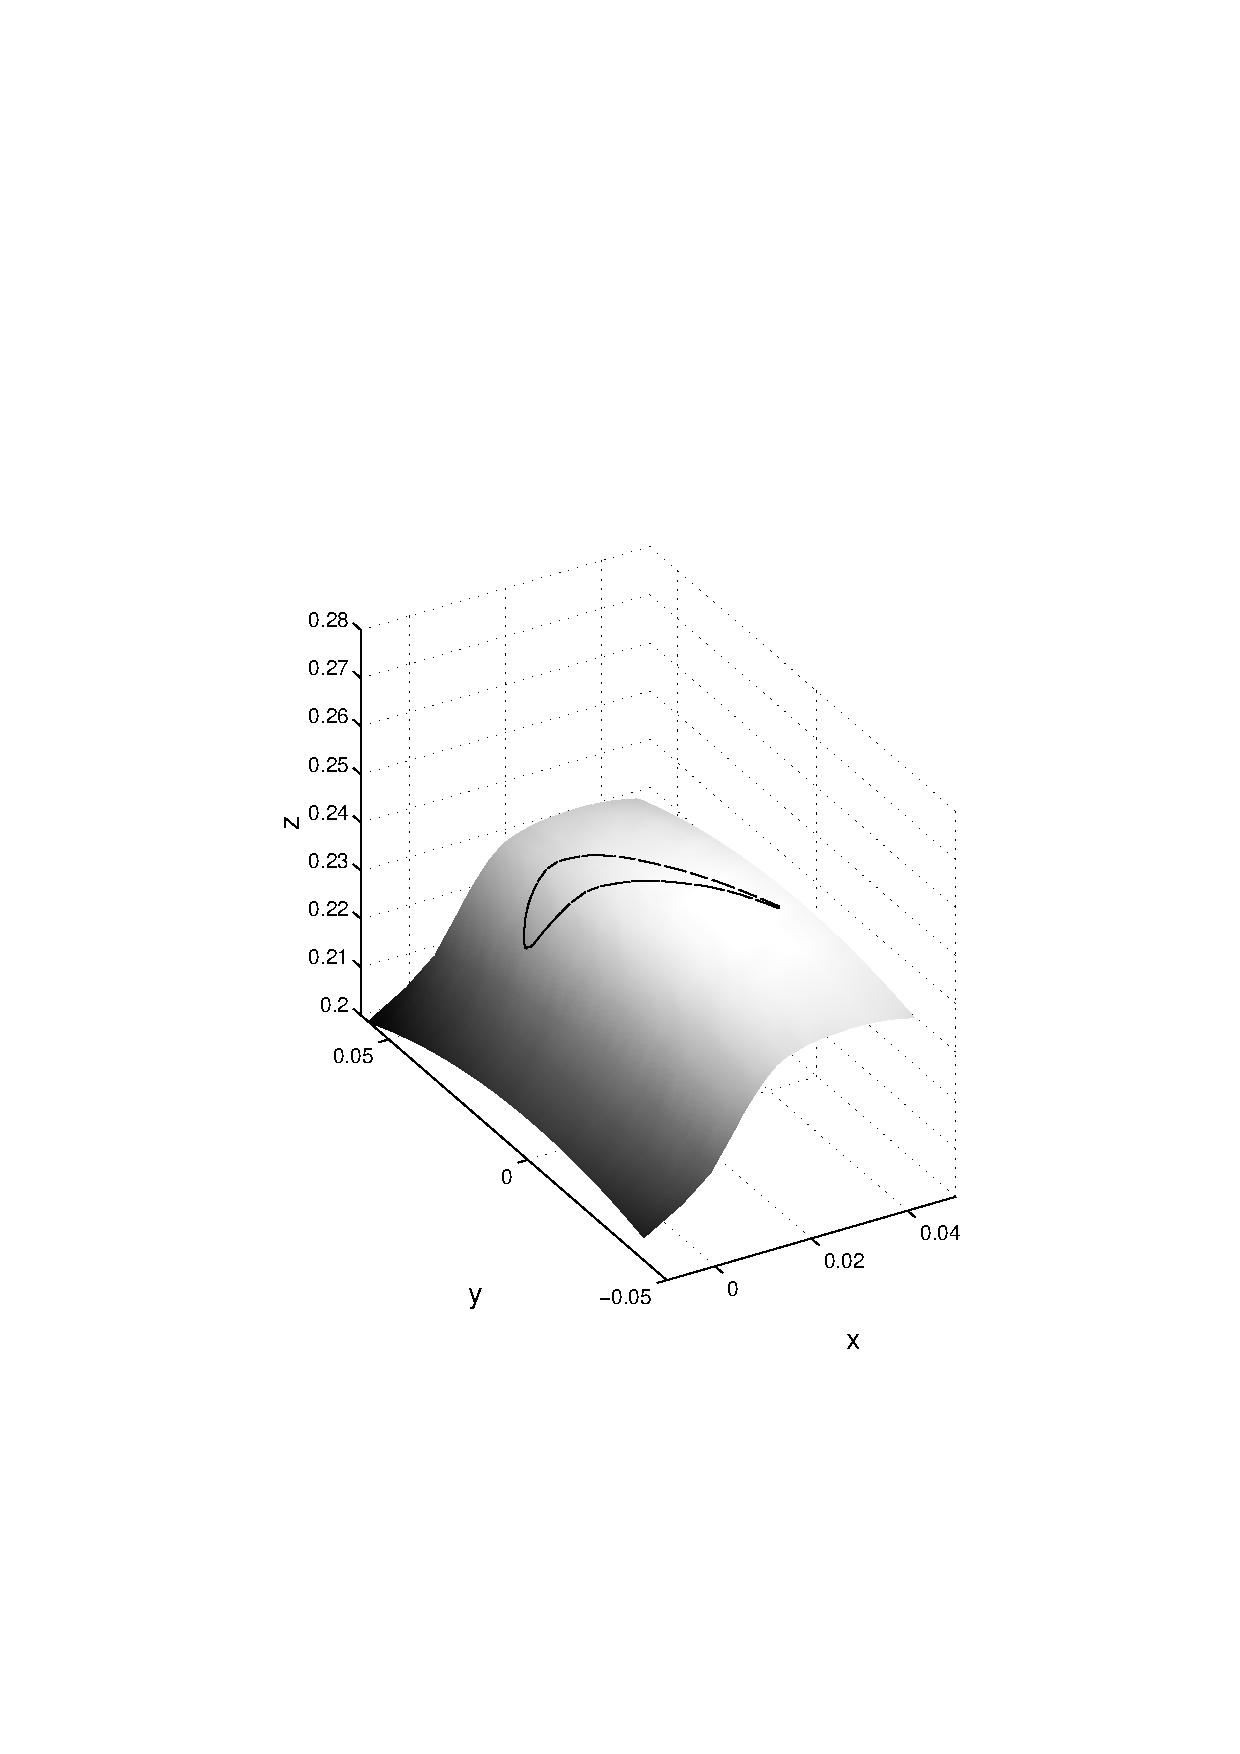
\includegraphics[width=70mm,clip=t]{CHAP_MESH/FIGURE/surf1.pdf}
      \hspace{0mm}}
    \subfigure[Hub-middle section (25\% span)]
      {\hspace{0mm}
       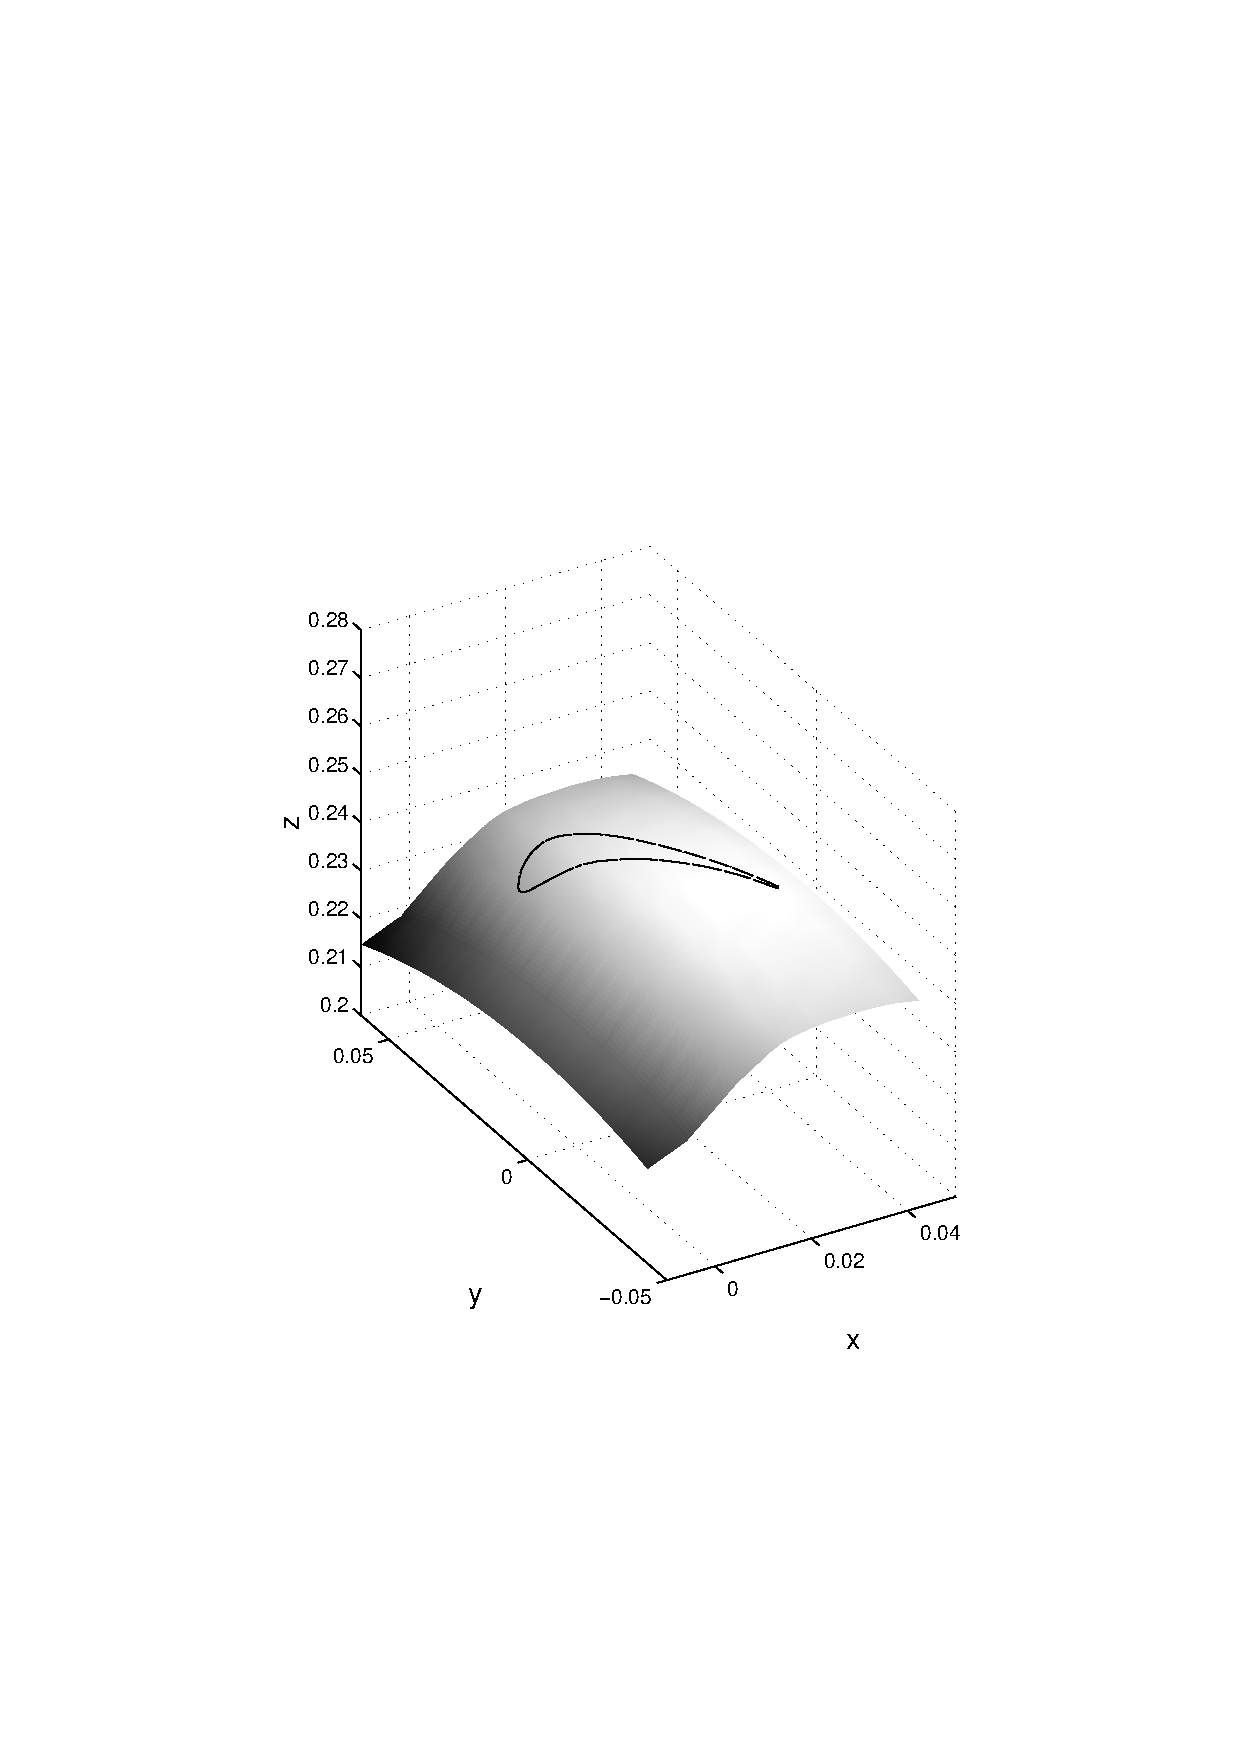
\includegraphics[width=70mm,clip=t]{CHAP_MESH/FIGURE/surf2.pdf}}
    \\
    \subfigure[Tip-middle section (75\% span)]
      {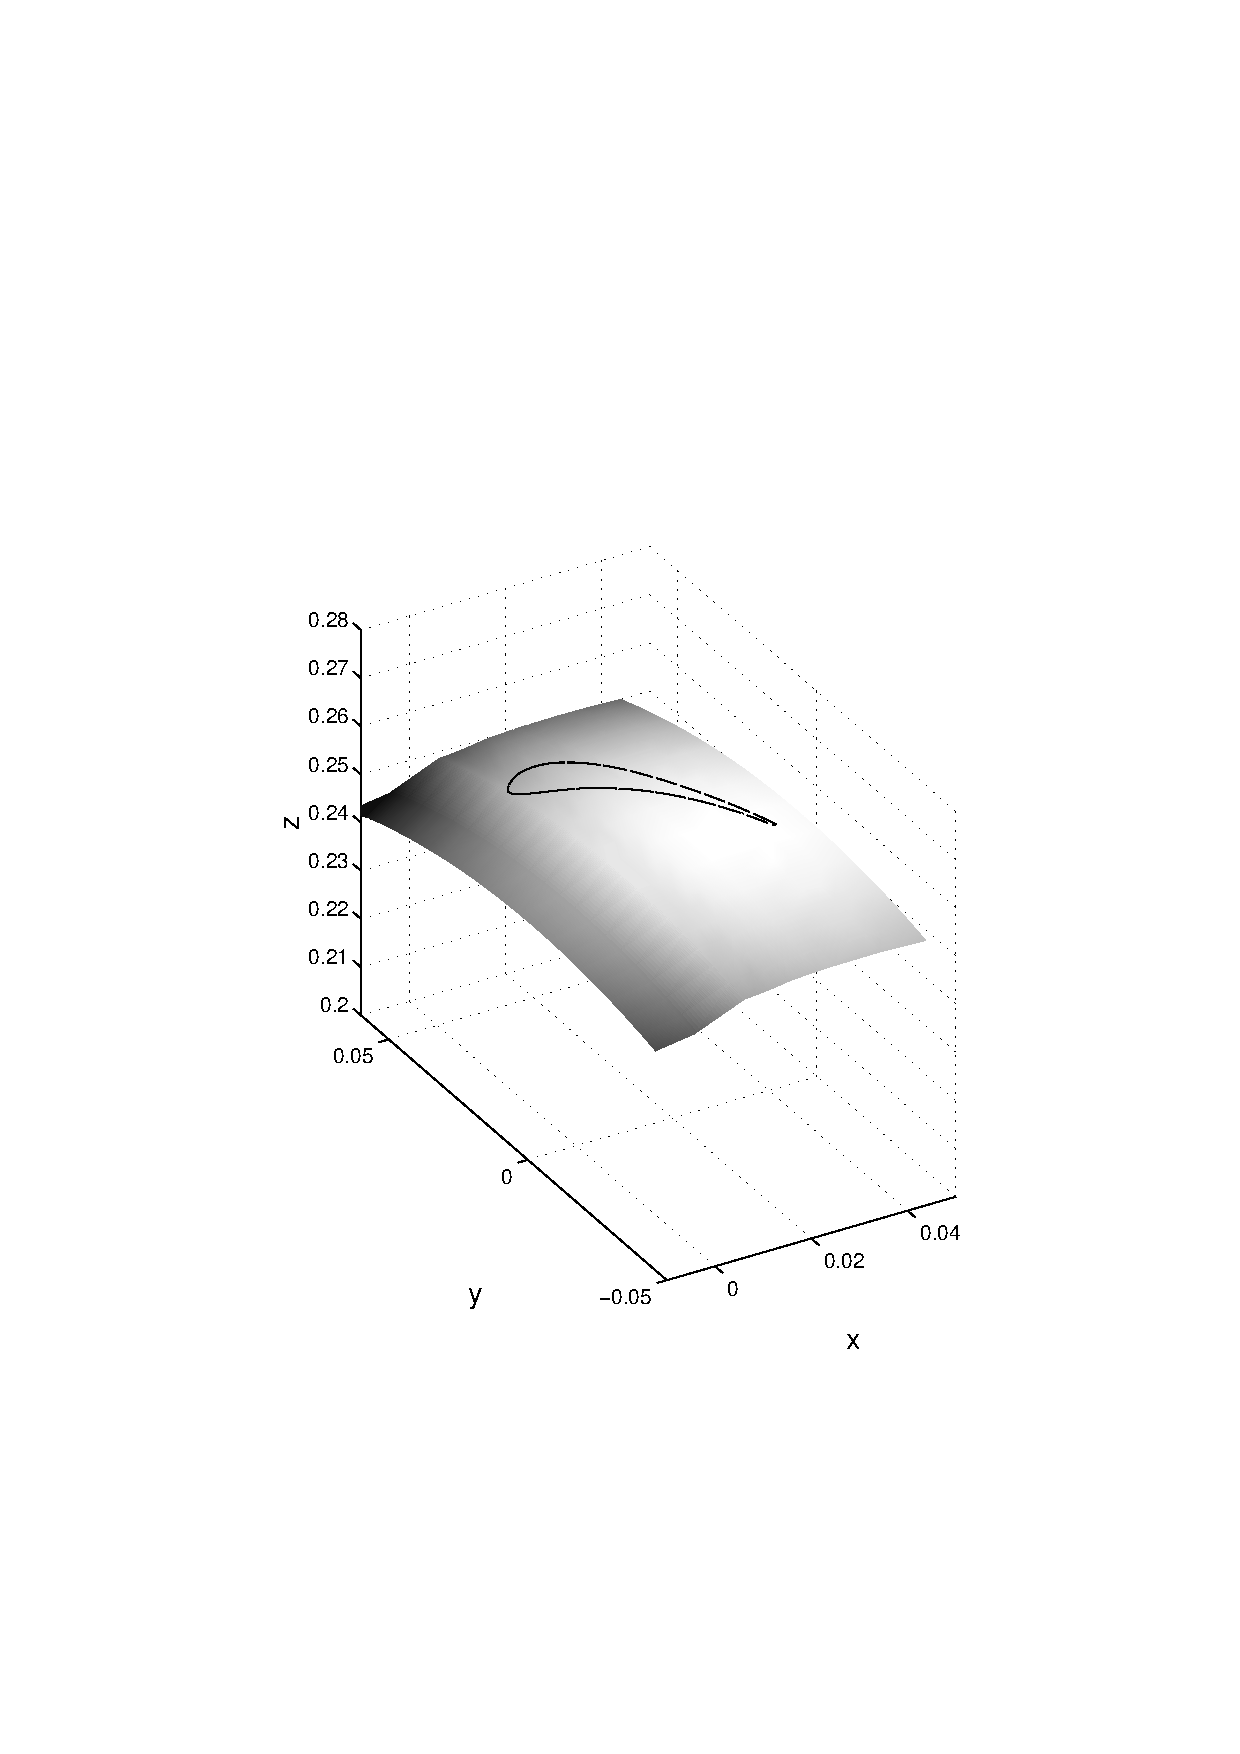
\includegraphics[width=70mm,clip=t]{CHAP_MESH/FIGURE/surf3.pdf}
      \hspace{0mm}}
    \subfigure[Tip section]
      {\hspace{0mm}
       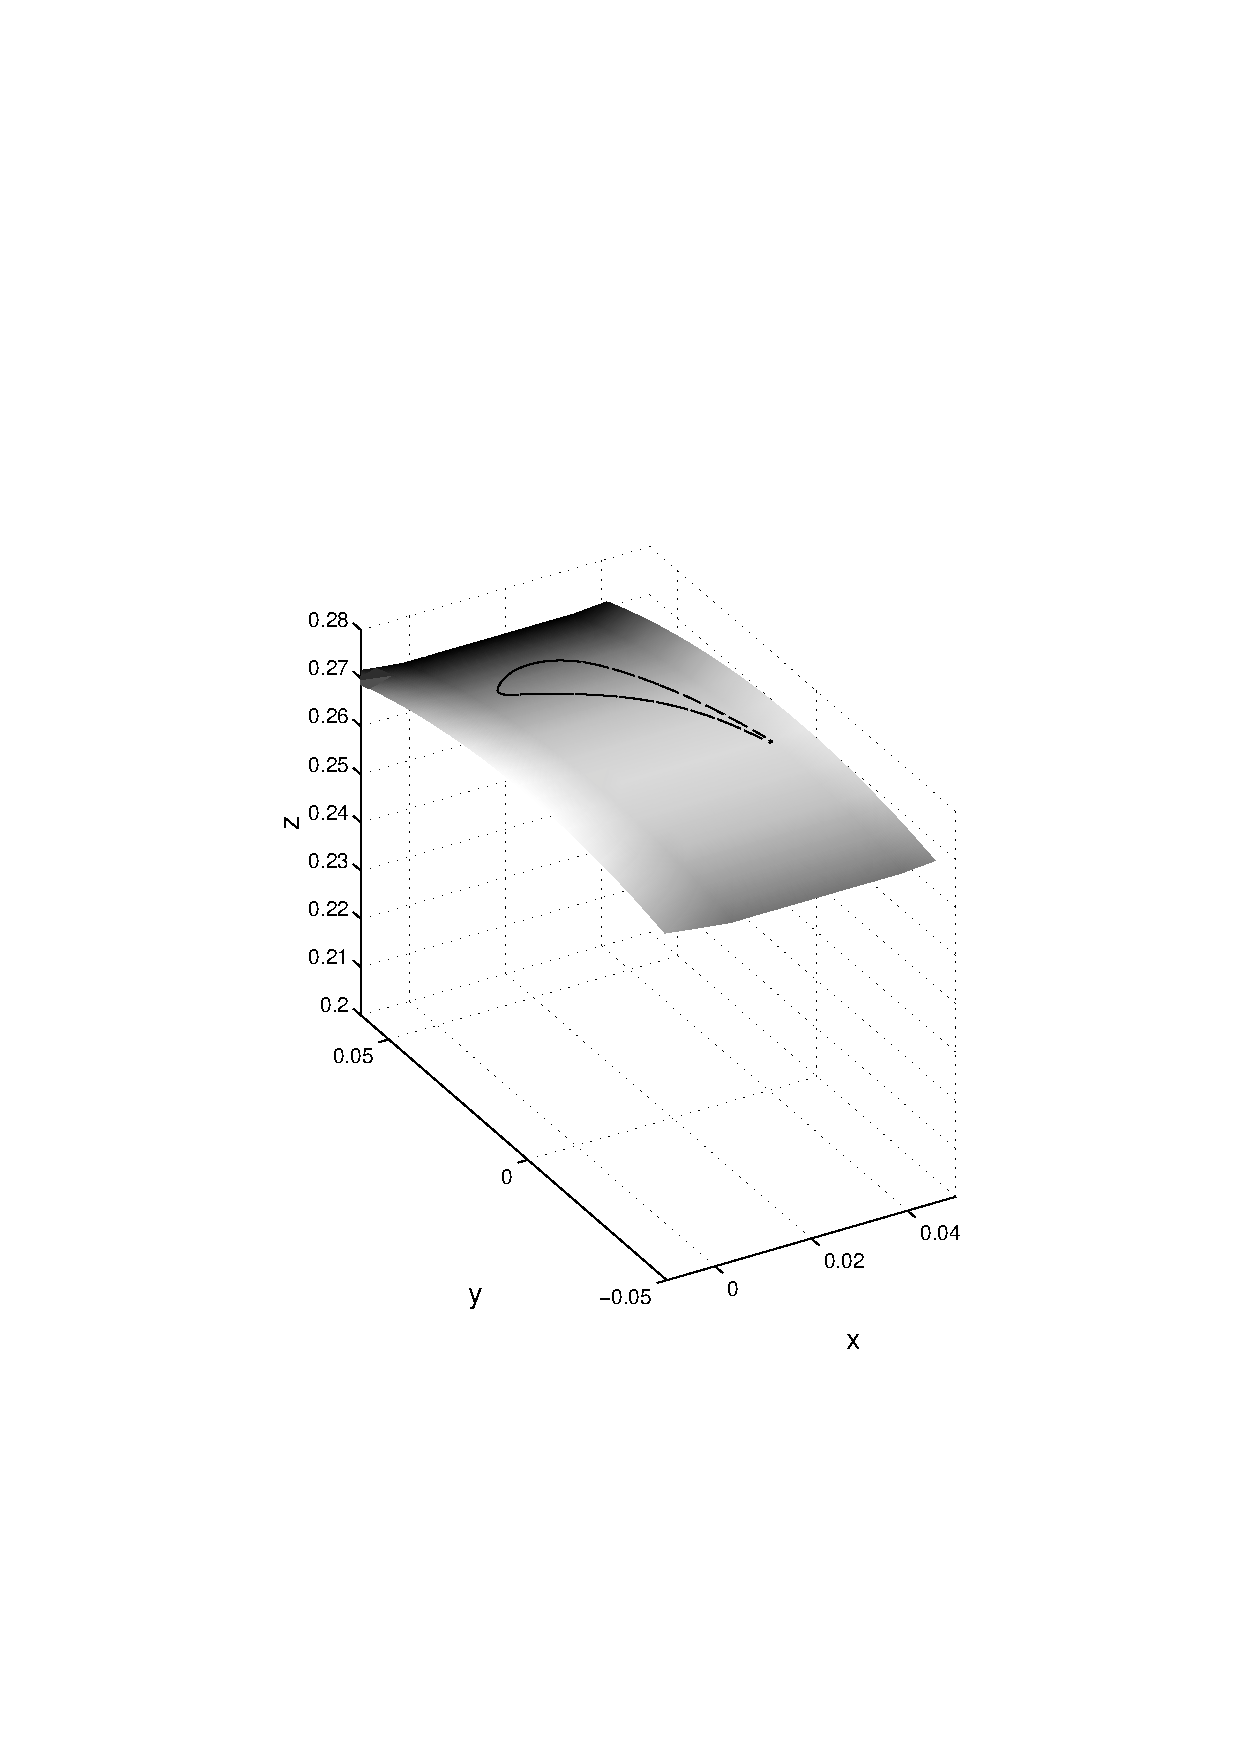
\includegraphics[width=70mm,clip=t]{CHAP_MESH/FIGURE/surf4.pdf}}
  \end{tabular}
 \end{center}
 \caption{Geometry definition of an NGV blade at different radial levels}
 \label{radial_levels.fig}
\end{figure}
%

 The starting point of the present method is the projection of
 the radial sections into parametric 2D planes,
 using the local coordinate system $u$ and $v$.
 In this way, the mesh-generation procedure will deal with
 plane sections only, thus the geometric dimension is reduced from
 three to two.
 Fig. \ref{radial_levels.fig} shows four different radial levels
 for a typical nozzle guide vane from a well-known aeroengine manufacturer.
 In this example
 $\sigma_i(x,r,\theta)$ is a surface of revolution around the $x$-axis, i.e.
 $r_{\sigma} = r\left(x\right)$.
 The parametric coordinates $u$ and $v$ are defined as:

%
\beq
  u  &=& \int\sm{x\sm{0}}\se{x} r\left(s\right) ds\\
  v  &=& r\left(x\right)\theta
\eeq
%
 Fig. \ref{radial_mapping.fig} shows the projection of the four radial
 levels shown in Fig. \ref{radial_levels.fig}.
%
\begin{figure}[ht]
 \begin{center}
  \begin{tabular}{cc}
    \subfigure[Hub section]
      {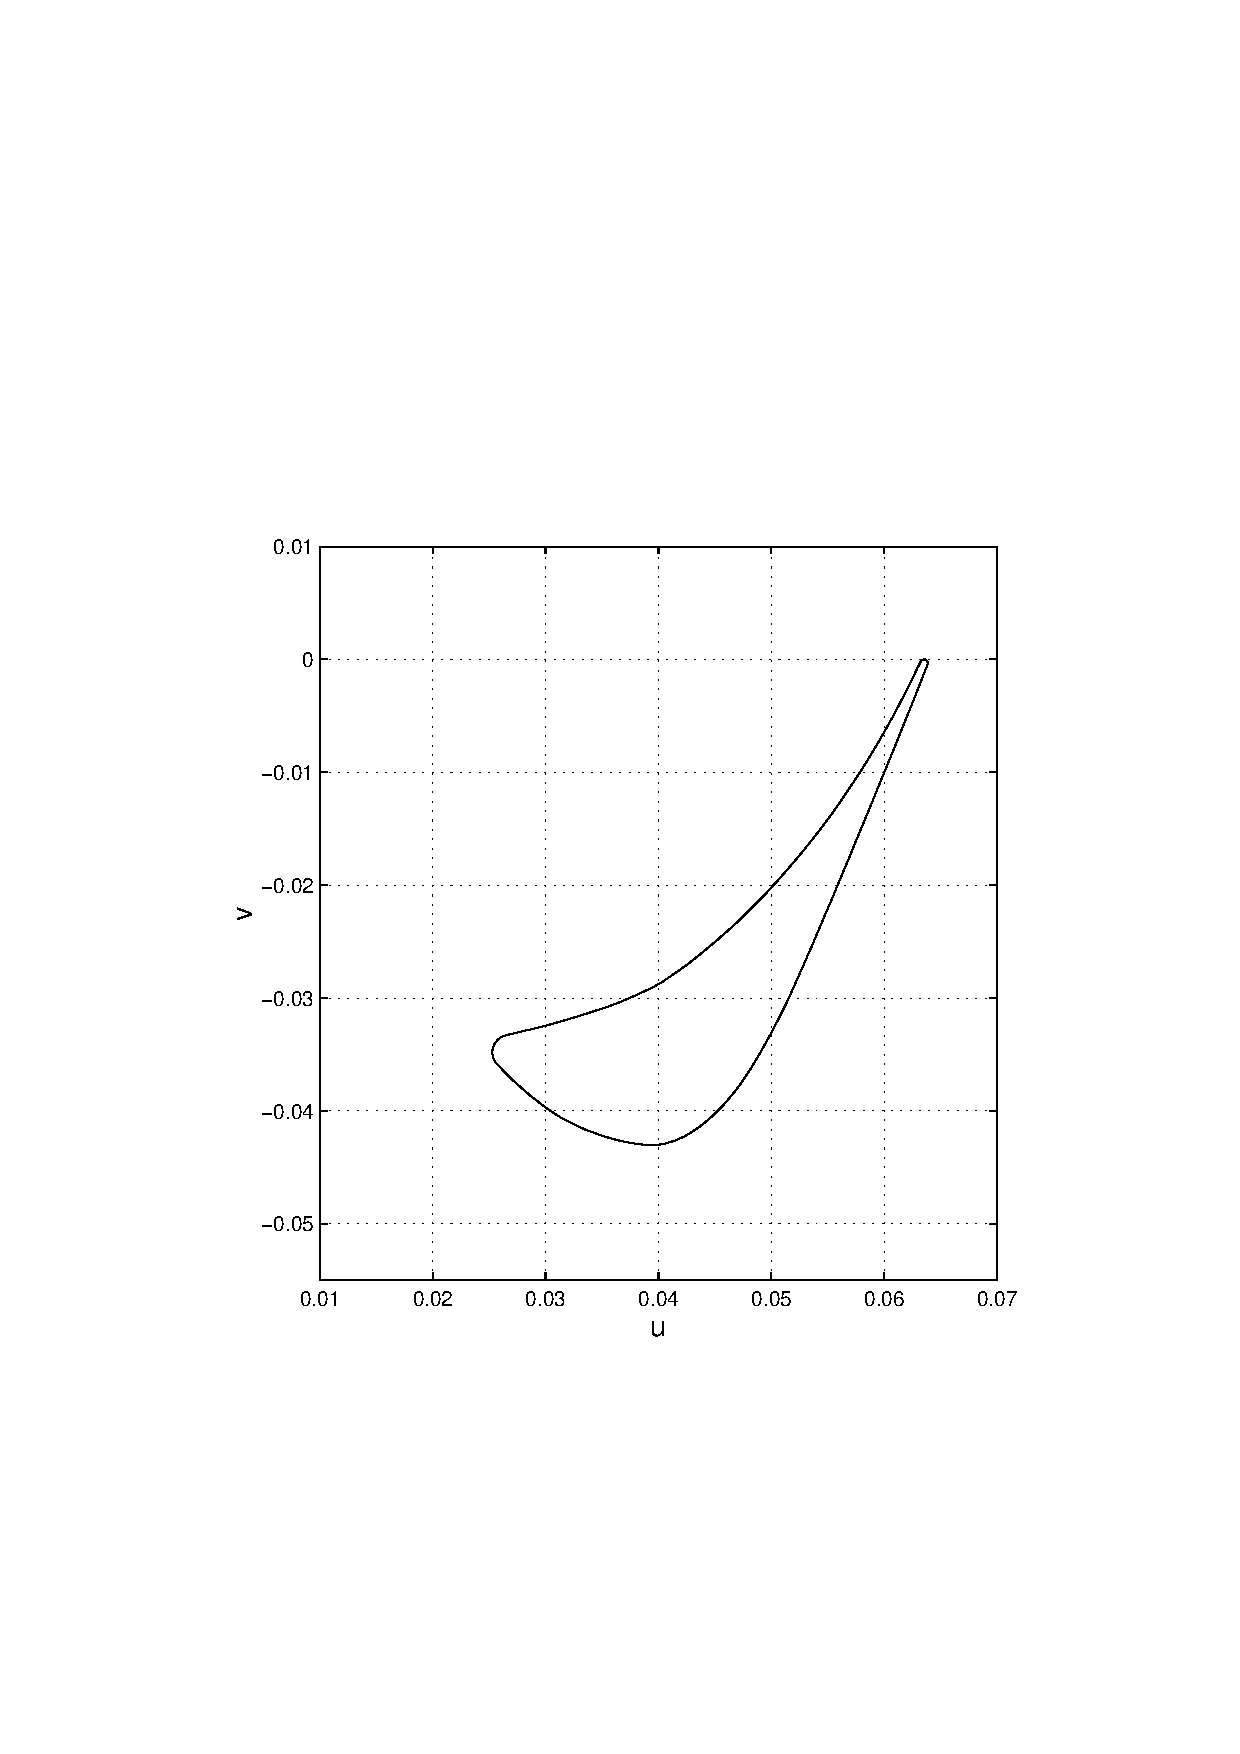
\includegraphics[width=50mm,clip=t]{CHAP_MESH/FIGURE/bla1.pdf}
      \hspace{10mm}}
    \subfigure[Hub-middle section (25\% span)]
      {\hspace{10mm}
       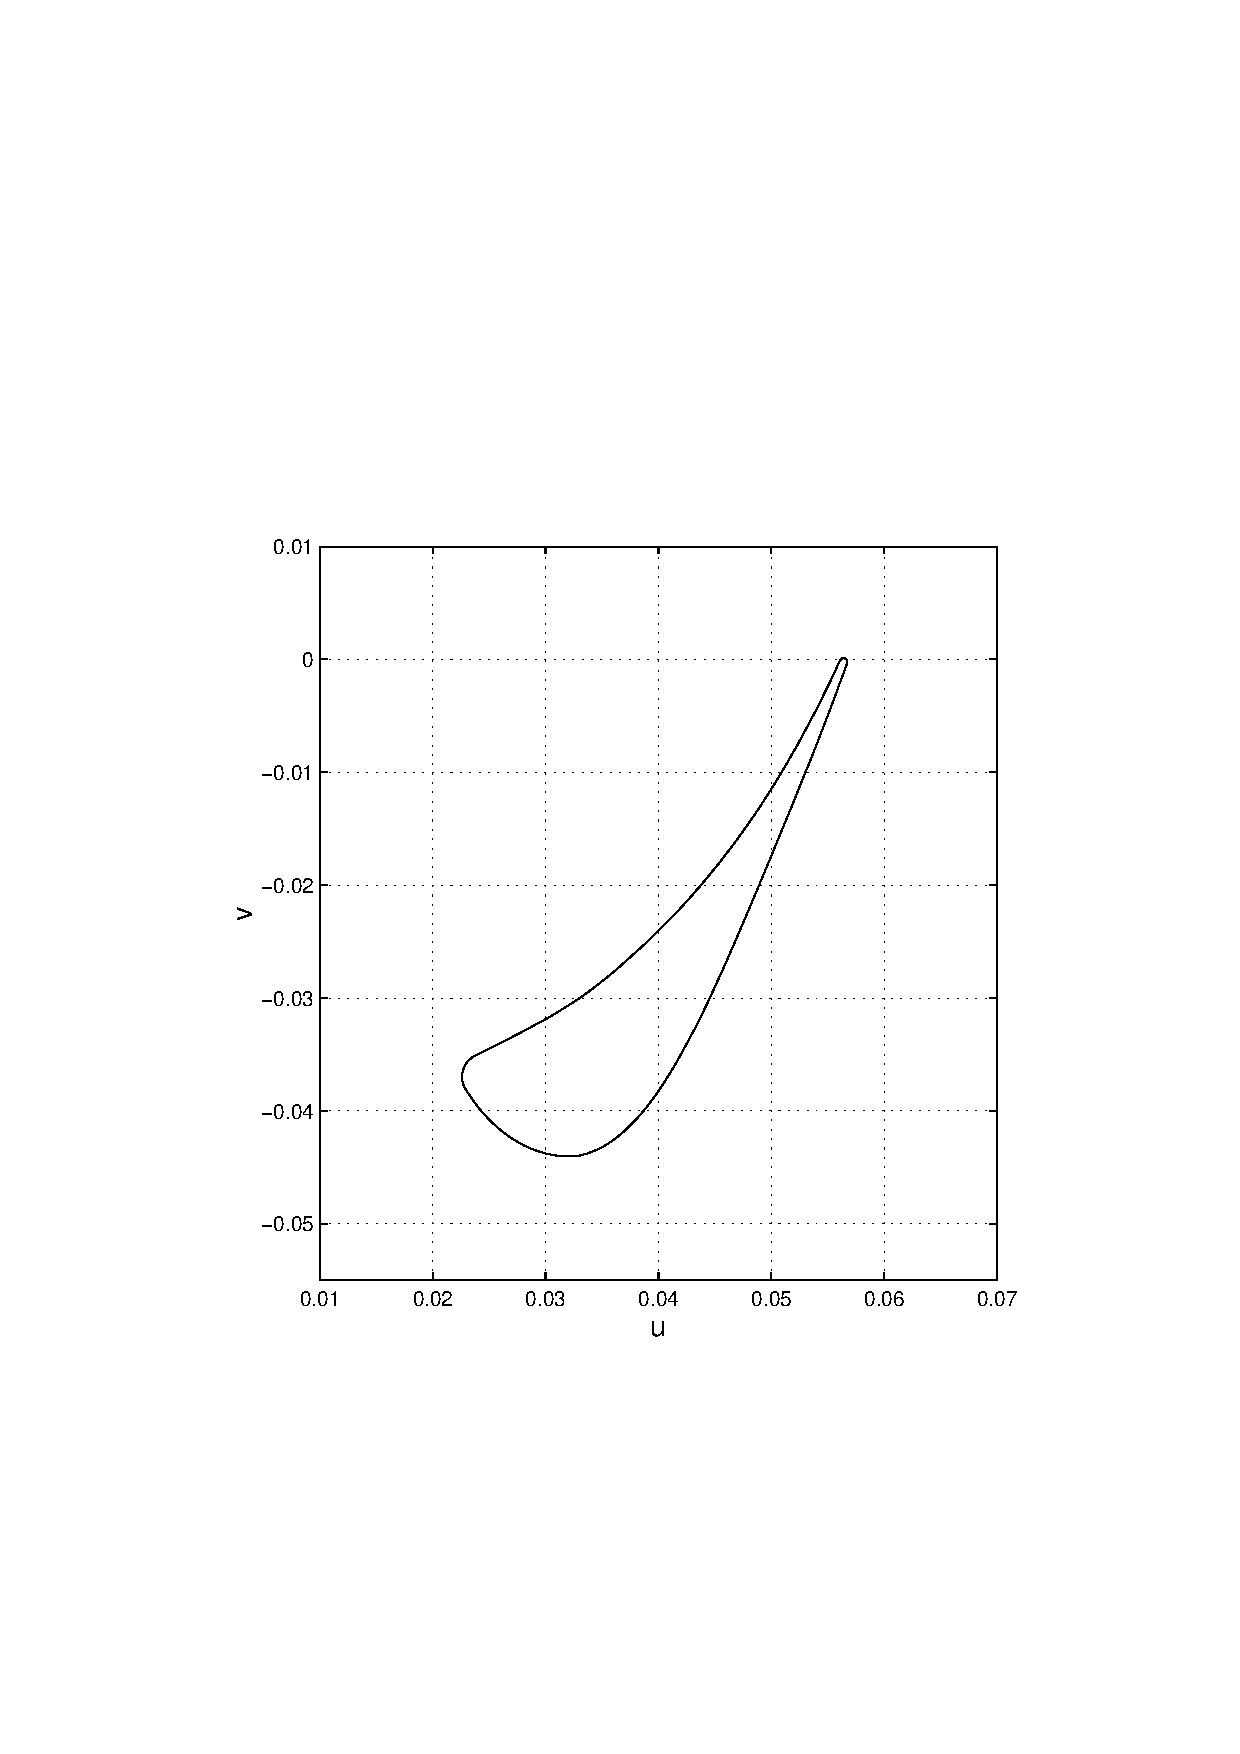
\includegraphics[width=50mm,clip=t]{CHAP_MESH/FIGURE/bla2.pdf}}
    \\
    \subfigure[Tip-middle section (75\% span)]
      {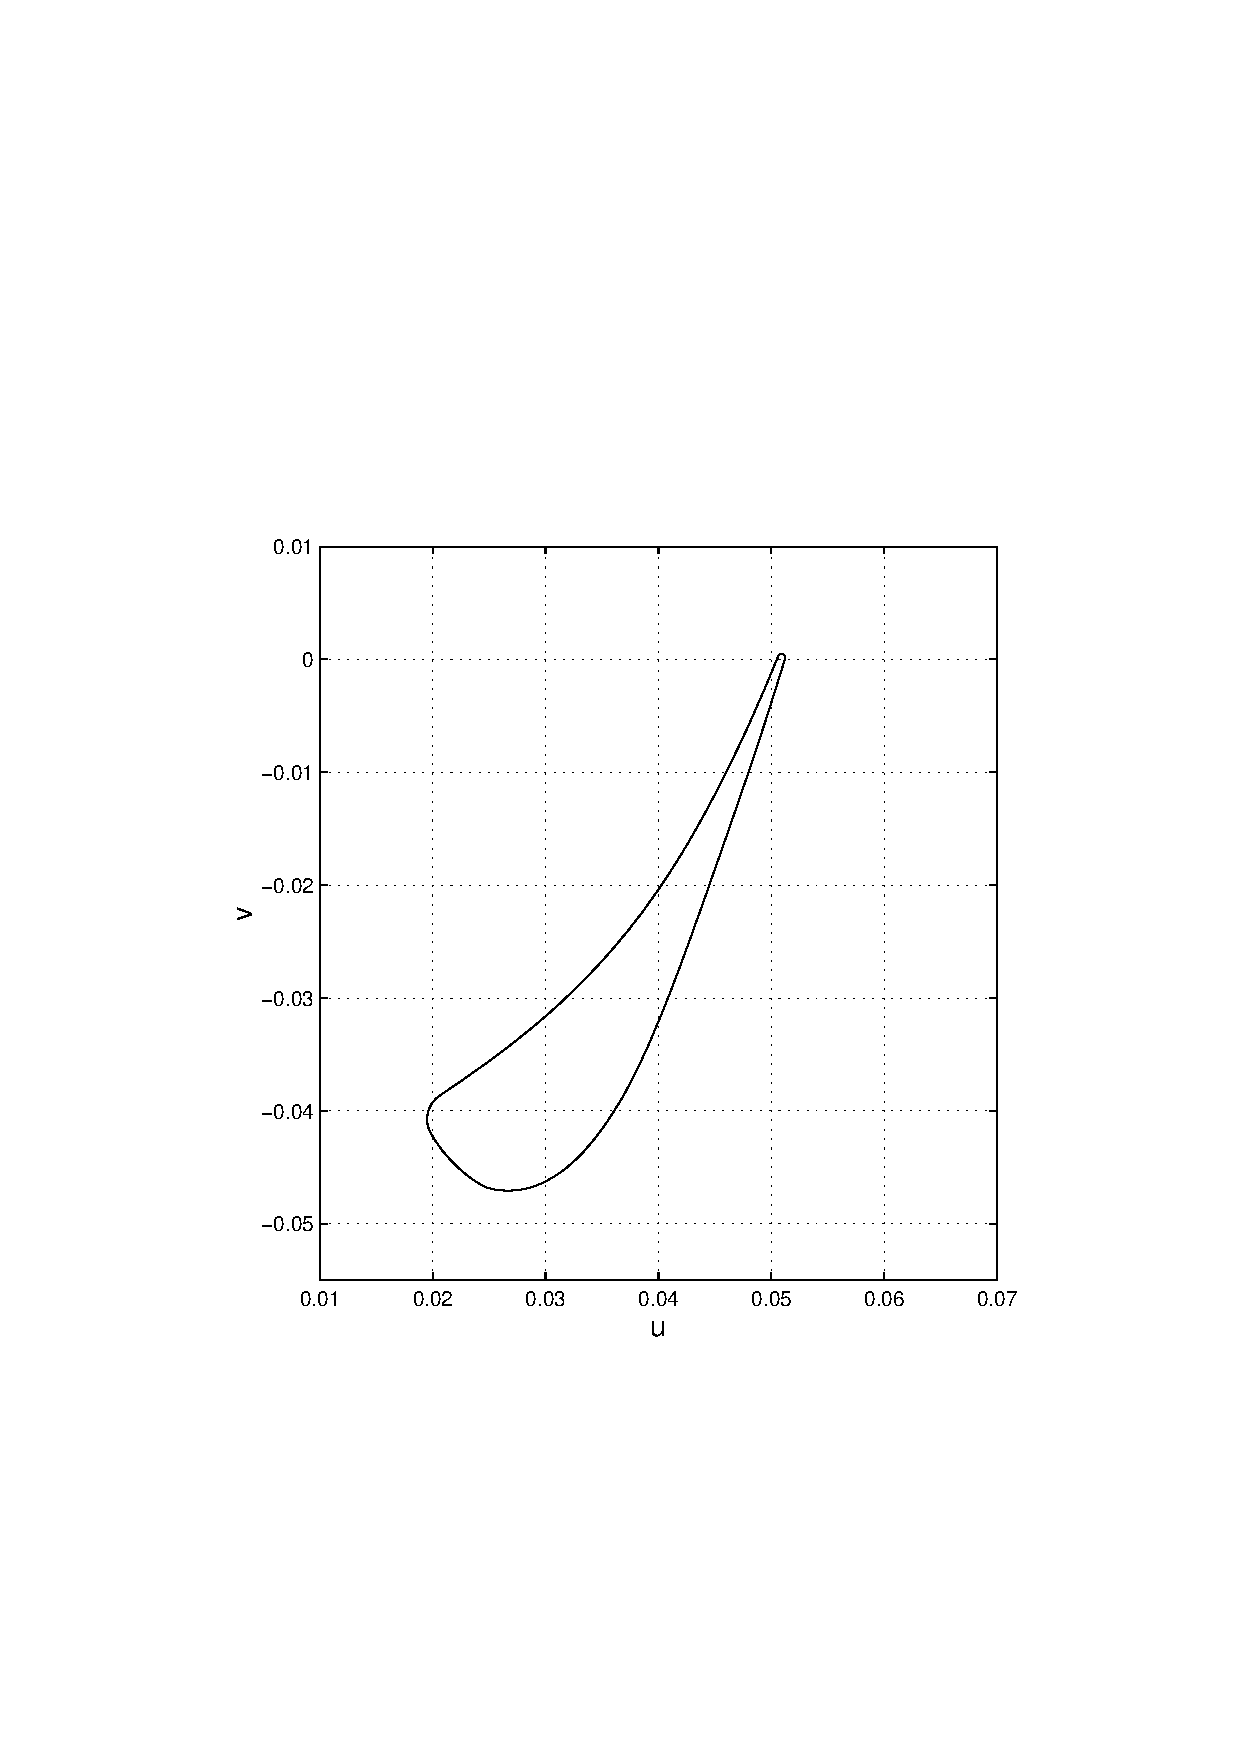
\includegraphics[width=50mm,clip=t]{CHAP_MESH/FIGURE/bla3.pdf}
      \hspace{10mm}}
    \subfigure[Tip section]
      {\hspace{10mm}
       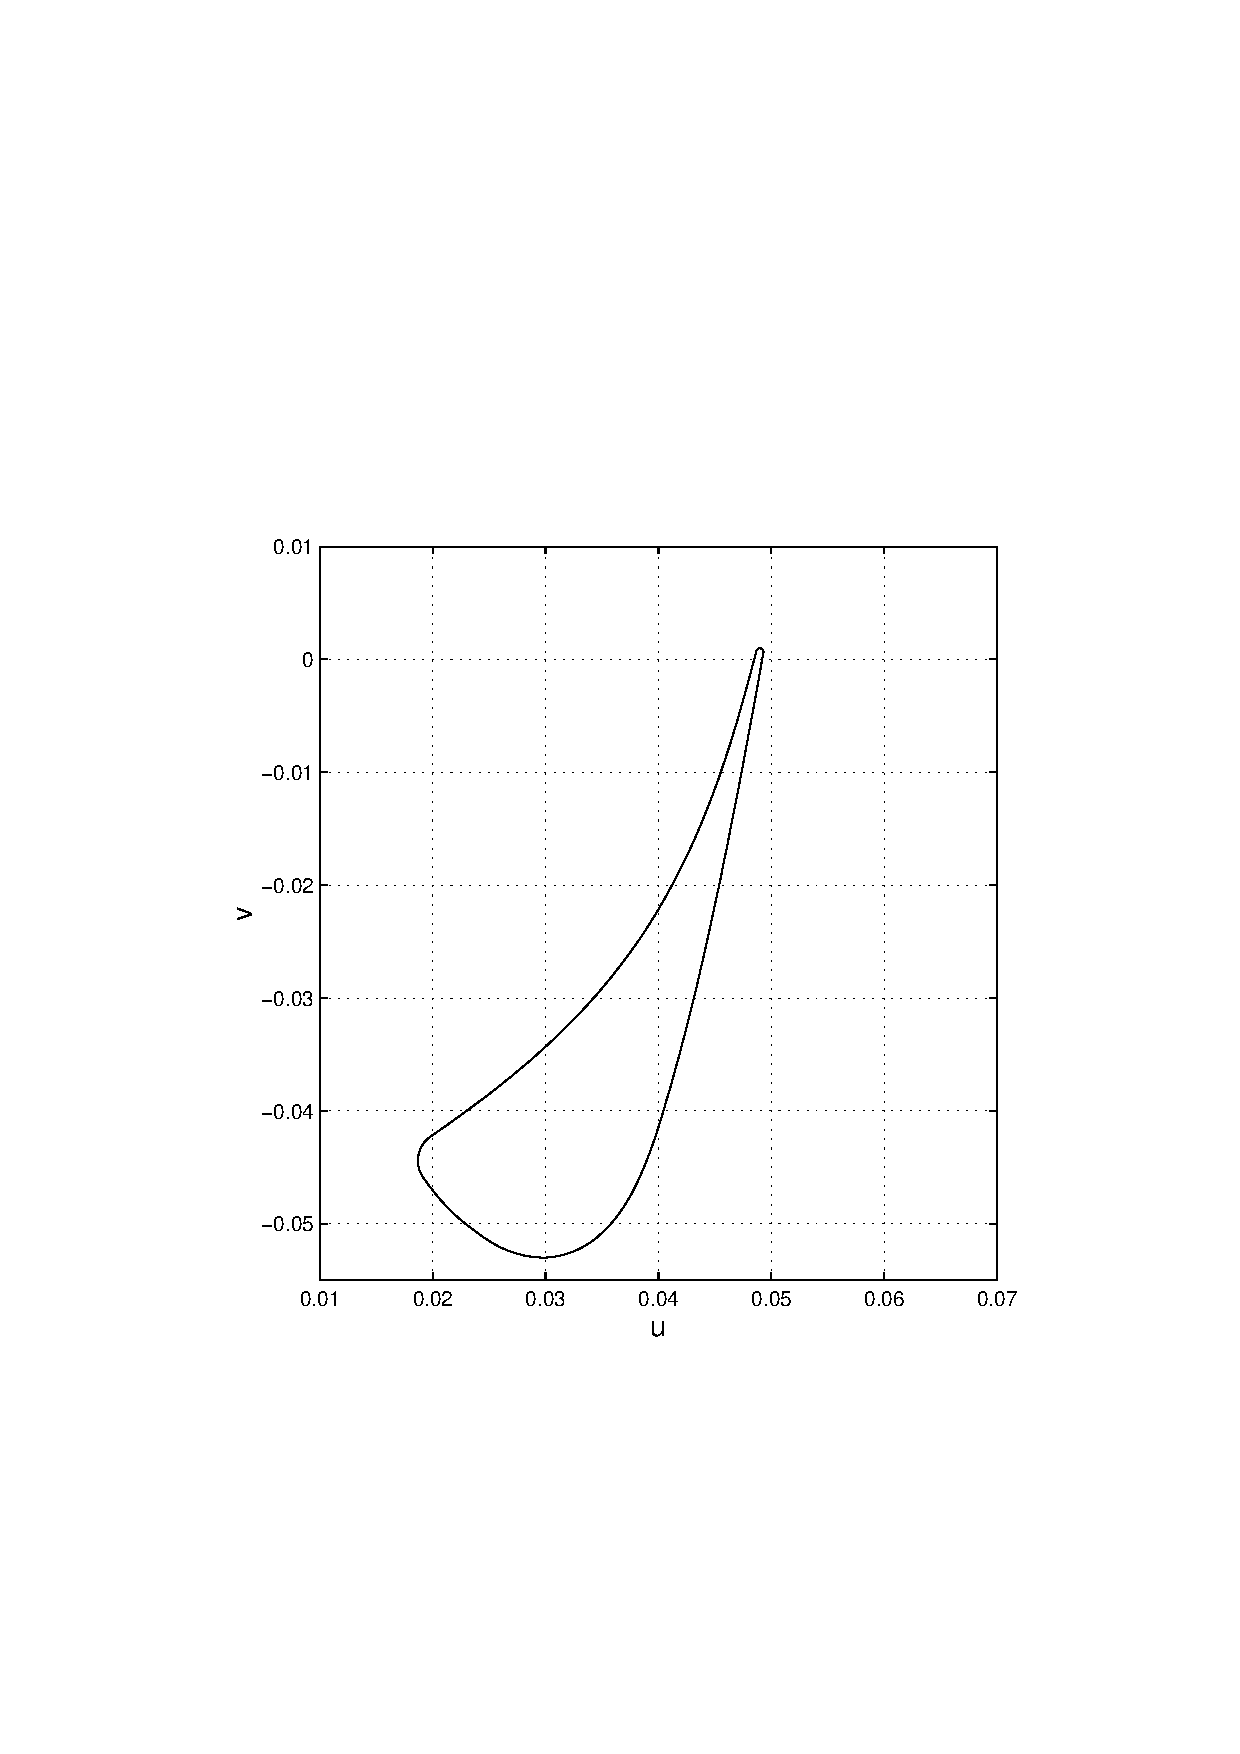
\includegraphics[width=50mm,clip=t]{CHAP_MESH/FIGURE/bla4.pdf}}
  \end{tabular}
 \end{center}
 \vspace{-5mm}
 \caption{Parametric 2D planes for four different radial levels}
 \label{radial_mapping.fig}
\end{figure}
%
%
\subsection{Unstructured mesh generation}
%
 Once all radial sections are projected into 2D planes,
 a hybrid quadrilateral-triangular mesh is generated in the 2D master plane
 which corresponds to a certain radial level (usually the middle one).
 The quadrilateral part of the mesh takes the form of a body-fitted
 O-grid which is generated using an advancing normal method.
 The orthogonality of this structured mesh is very important for
 an accurate resolution of the turbulent-boundary layer which
 originates from high Reynolds number flows. This point will be
 stressed further in the next chapter where a novel finite-volume discretisation
 of the Navier-Stokes equations on hybrid grids will be explored.
 The remaining part of the domain is discretised using an unstructured
 mesh generator which uses an advancing front algorithm (Morgan et al.
 \citeyearNP{Peiro:1}, Mavriplis \citeyearNP{Mavriplis:2}).
 A distinctive feature of this method is that both triangles and
 points are generated simultaneously.
 Such an approach enables the generation of elements
 with variable sizes and stretching, and hence it differs from Delaunay-type
 mesh generators (Baker \citeyearNP{Delaunay},
 Mavriplis \citeyearNP{Mavriplis:2}).

 Fig. \ref{mesh2d_master.fig}b shows the final unstructured hybrid-grid
 of the NGV in Fig. \ref{radial_levels.fig}
 in the 2D master plane which, in this case, corresponds to the projected
 middle section of the 3D blade.

%
%
\subsection{Quasi-conformal mapping}
%
 An important part of the mesh-generation strategy is
 the mapping procedure to project the 2D unstructured mesh of
 the master plane back to all radial blade-definition levels.
 A necessary condition for a mapping function is that
 it must associate a given point of the master plane with one,
 and only one, point of the target plane.
 Moreover a mapping function should also guarantee
 that a given angle in the master plane is mapped into a similar-valued angle
 in the target plane (quasi-conformal mapping). This last property is essential
 in order to minimize the skewness of the mesh, especially for
 highly-twisted blades.

 The starting point for the quasi-conformal mapping is the generation
 of coarse structured quadrilateral grids for all projected radial levels,
 including the master plane.
 Following the approach of Steger \& Sorenson \citeyear{Ellipt2},
 these meshes are obtained by solving a system of elliptic partial-differential
 equations.
 An essential requirement for such structured meshes is that they must
 be generated in exactly the same manner, i.e. with the same number of
 points and quadrilaterals for all radial levels.
 Fig. \ref{mesh2d_master.fig} shows the structured quadrilateral grid
 and the unstructured hybrid-grid in the master plane, which correspond
 to the middle radial section.
%
\begin{figure}[ht]
 \begin{center}
  \begin{tabular}{cc}
    \subfigure[Structured mesh for mapping]
      {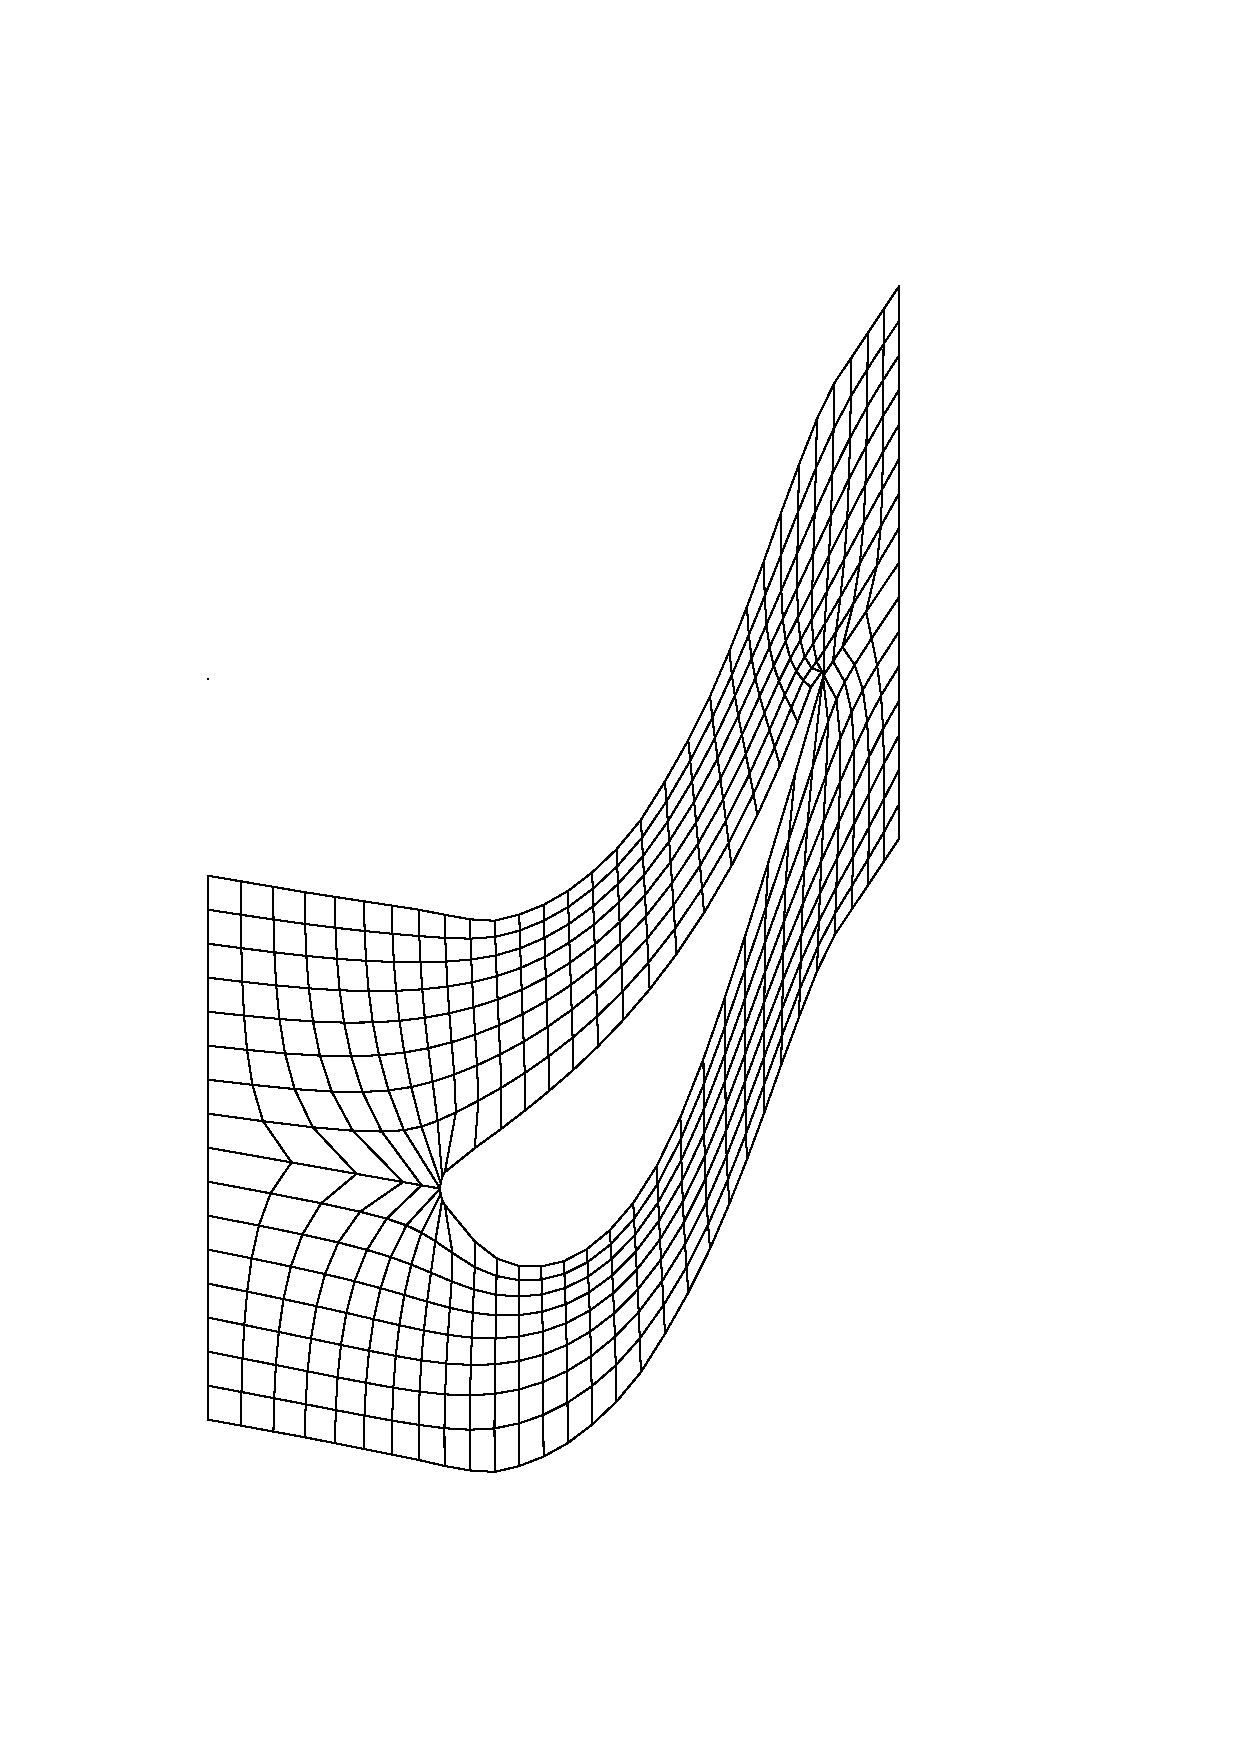
\includegraphics[width=70mm,clip=t]{CHAP_MESH/FIGURE/mesh2d_struct.pdf}}
    \subfigure[Unstructured mesh]
      {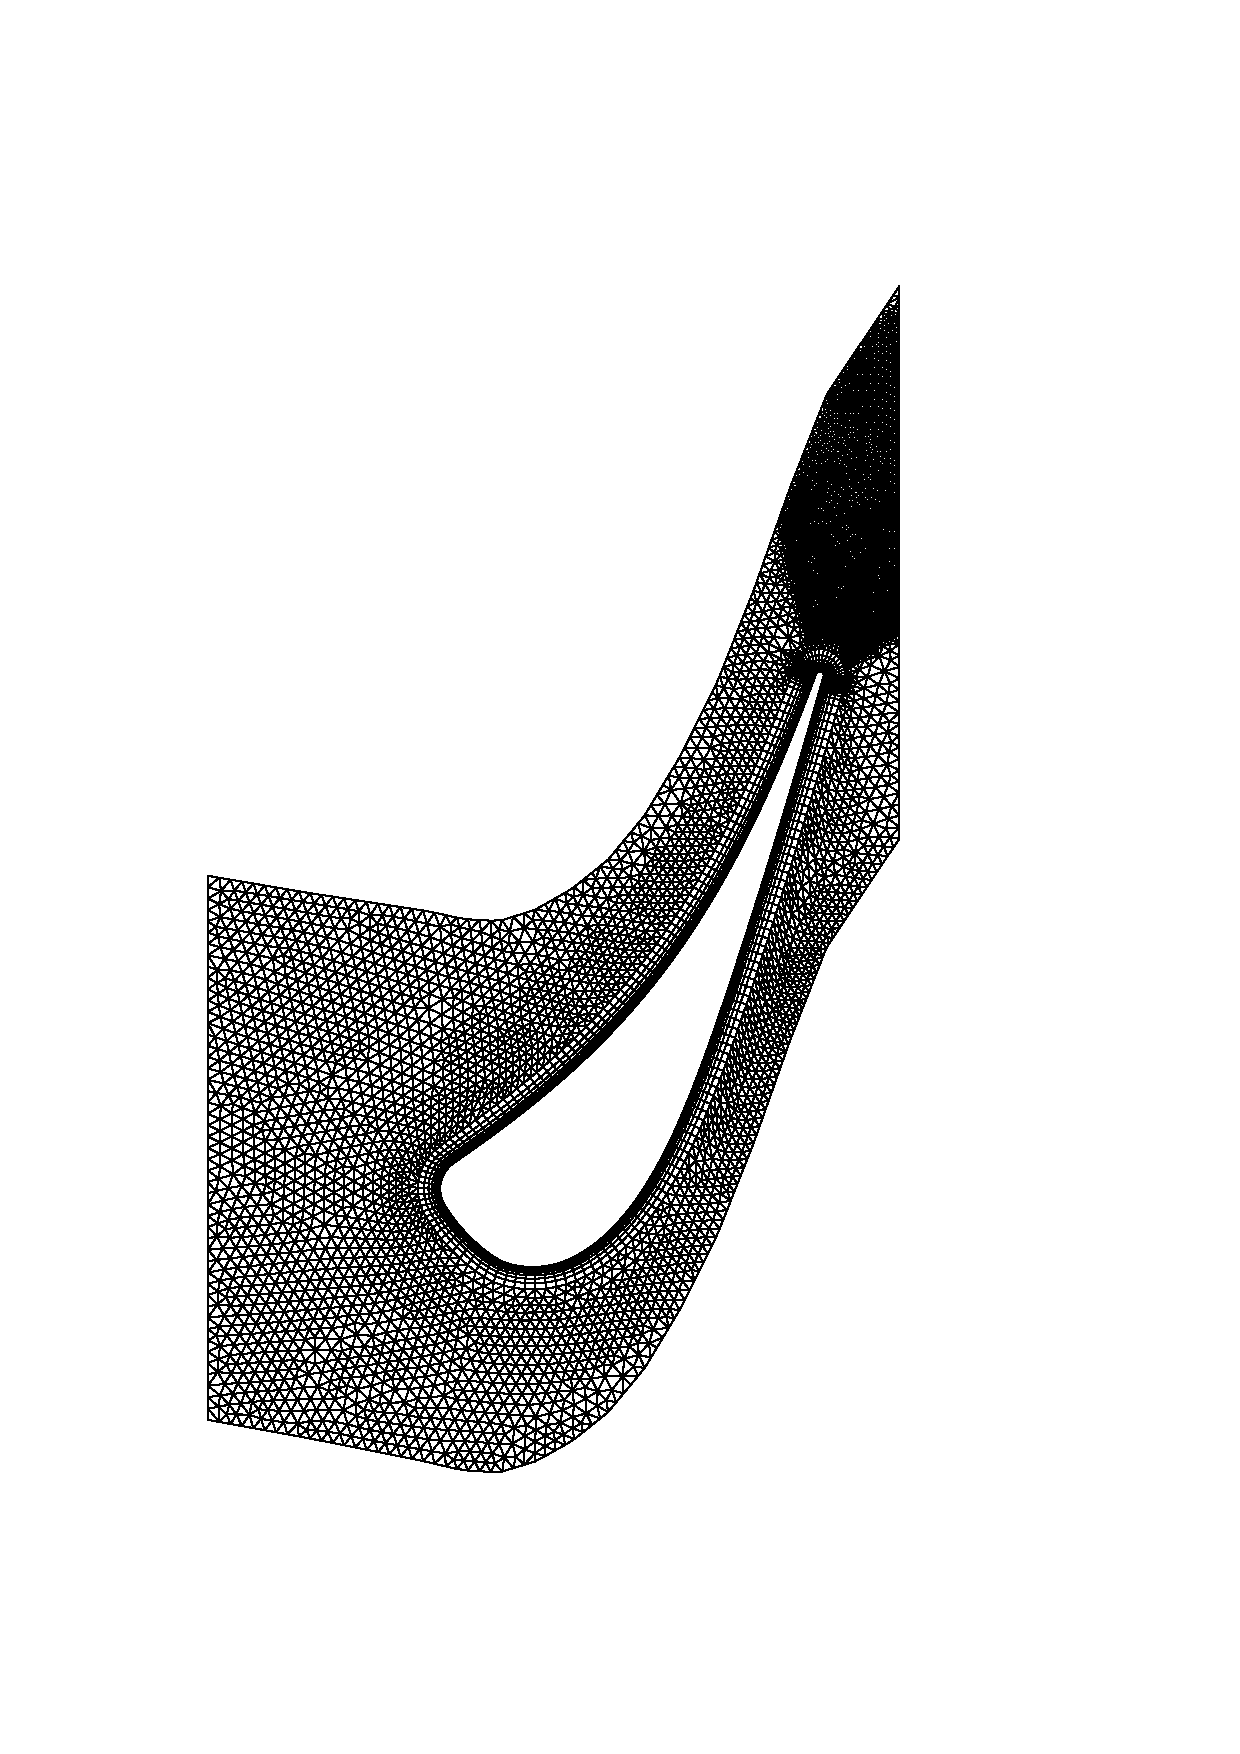
\includegraphics[width=70mm,clip=t]{CHAP_MESH/FIGURE/mesh2d_unstruct.pdf}}
  \end{tabular}
 \end{center}
 \vspace{-5mm}
 \caption{Meshes in the master plane}
 \label{mesh2d_master.fig}
\end{figure}
%
 The mapping procedure is divided into three different steps.
%
\paragraph{\bf Geometry searching in the master plane.}
 Each point $J$ of the unstructured 2D mesh in Fig \ref{mesh2d_master.fig}b
 must be located on quadrilateral $E$ of the structured mesh in
 Fig \ref{mesh2d_master.fig}a.
%
 \paragraph{\bf Inverse mapping in the master plane.}
 The Cartesian coordinates
 $\vec{x}\sm{J} = \left(x\sm{J}, y\sm{J}\right)$ of point $J$,
 associated with the quadrilateral $E$ are given by
%
\begin{equation}
  \vec{x}\sm{J} = \sum_{I=1}^4 \vec{x}\sm{I}
                   N\sm{I} \left(\xi\sm{J},\eta\sm{J}\right)
  \label{mapping_1}
\end{equation}
%
 where $\left(\xi\sm{J},\eta\sm{J}\right)$ represent the local-coordinates,
 $\vec{x}\sm{I}$ represents the Cartesian coordinates of nodes $I=1,\dots,4$
 of the quadrilateral $E$ and
 $N\sm{I}$ is the standard finite-element bilinear shape-function
 which takes the form (Zienkiewicz \& Morgan \citeyearNP{Zienk:1}):
%
\begin{equation}
  N\sm{I} = \frac{1}{4} \left\{
  \begin{array}{l}
     \left(1 - \xi\right) \left(1 - \eta\right) \\
     \left(1 + \xi\right) \left(1 - \eta\right) \\
     \left(1 + \xi\right) \left(1 + \eta\right) \\
     \left(1 - \xi\right) \left(1 + \eta\right)
  \end{array}
  \right.
  \label{shape_function}
\end{equation}
%
 A Newton-Raphson method is used in order to obtain the values of
 $\xi\sm{J}$ and $\eta\sm{J}$.
%
 \paragraph{\bf Direct mapping.}
 Once all points $J$ of the
 unstructured mesh in the master plane are associated with quadrilateral
 $E$ and local-coordinates $\left(\xi\sm{J},\eta\sm{J}\right)$
 are determined, coordinates $\vec{x}\sm{J}$ of points
 on the remaining projected radial sections are obtained
 directly using equation (\ref{mapping_1}).
\vspace{5mm}

 The above-described steps are shown in Fig. \ref{mapping.fig}.
%
\begin{figure}[ht]
   \centerline{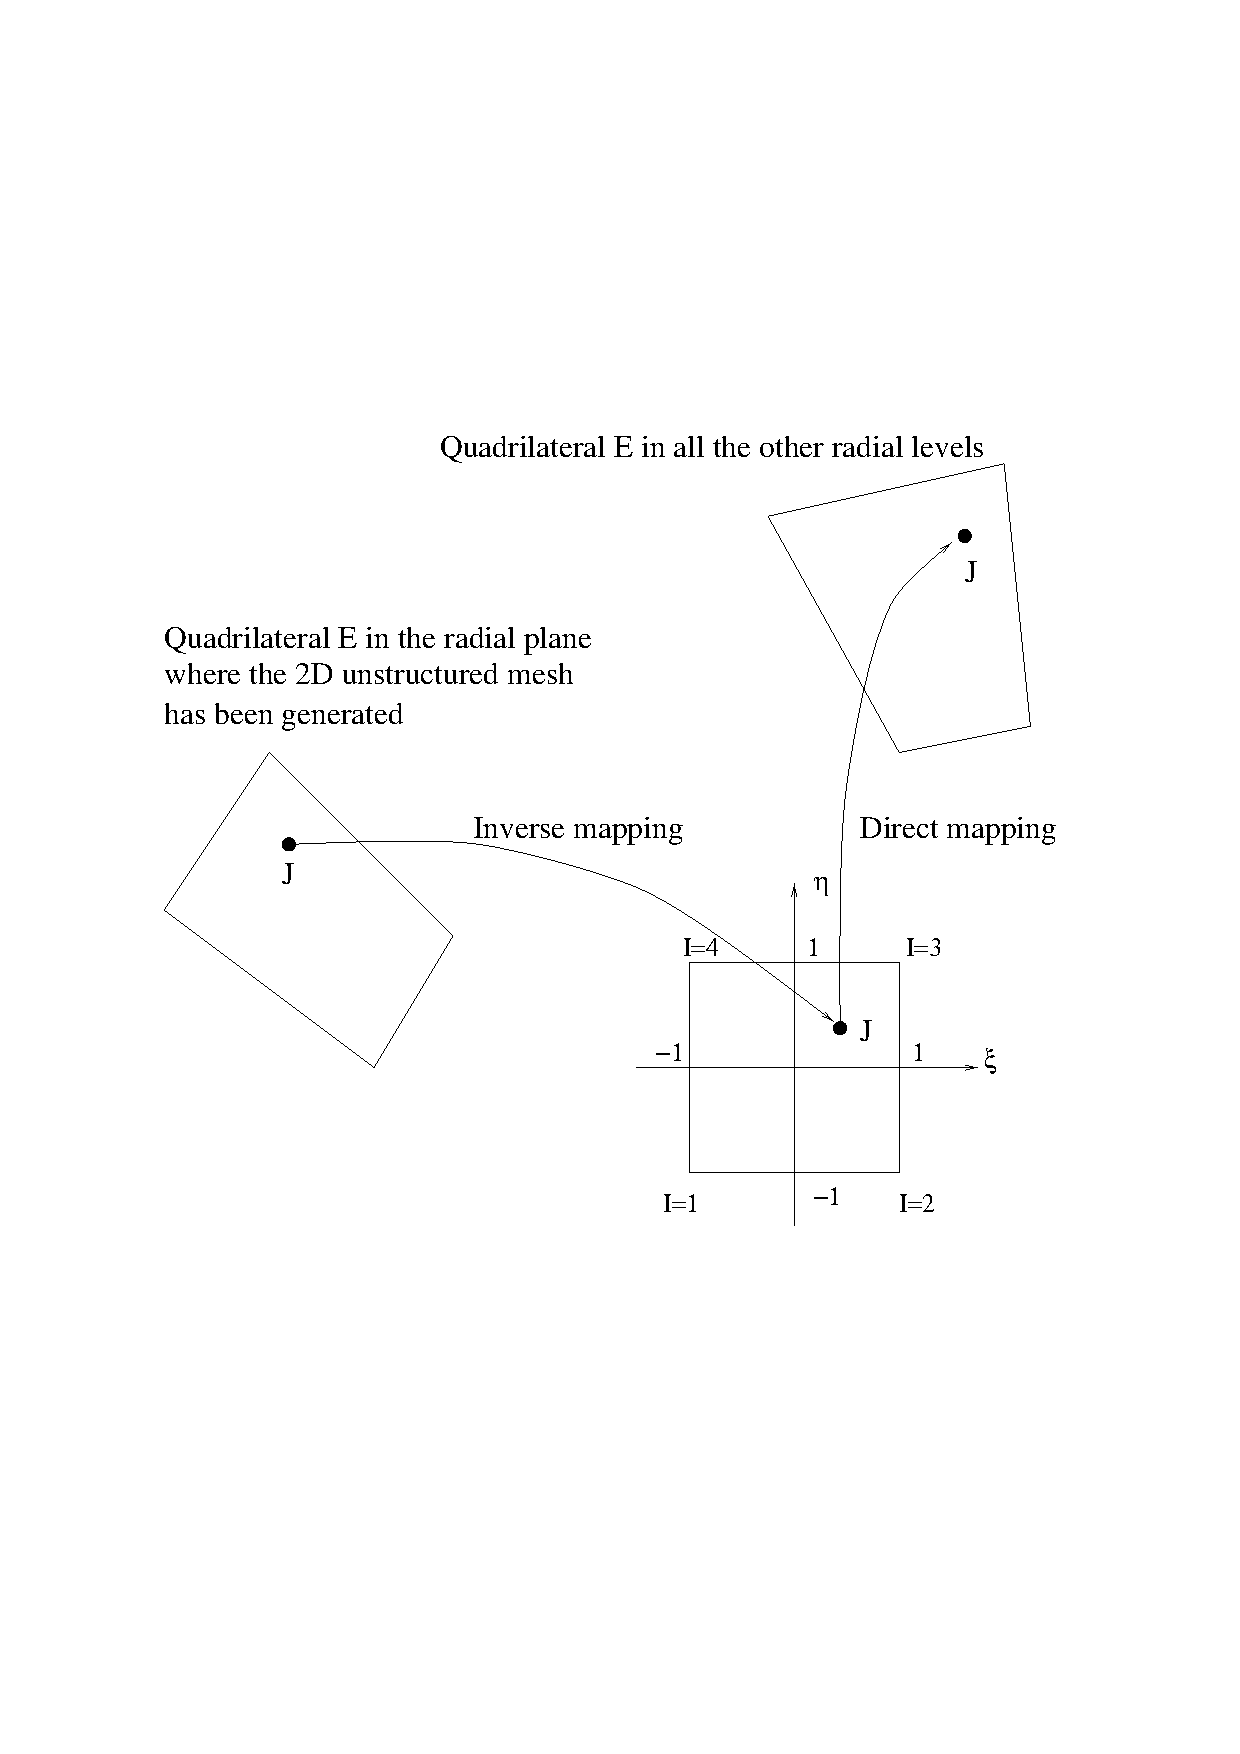
\includegraphics[width=120mm,clip=t]{CHAP_MESH/FIGURE/mapping.pdf}}
   \caption{Mapping procedure}
   \label{mapping.fig}
\end{figure}
%
 The mapping method becomes fully conformal if (i) a given element of the 2D
 hybrid mesh lies within a single quadrilateral of the structured
 grid. (ii) In addition, the angles of this quadrilateral must remain the
 same for all radial sections.
 If the above two conditions are not
 satisfied, the conformal property is not guaranteed and, for this reason,
 the procedure has been labelled quasi-conformal here.
 Finally, it is worth noting that the algorithm is not CPU-intensive,
 since the geometry searching and
 the inverse-mapping are performed once only.

 Fig. \ref{mesh2d_other.fig} shows the structured meshes used for mapping
 and the corresponding mapped unstructured hybrid-grids at three radial levels.
%
\begin{figure}
 \begin{center}
  \begin{tabular}{c}
    \subfigure[Hub section]
      {\begin{tabular}{cc}
      {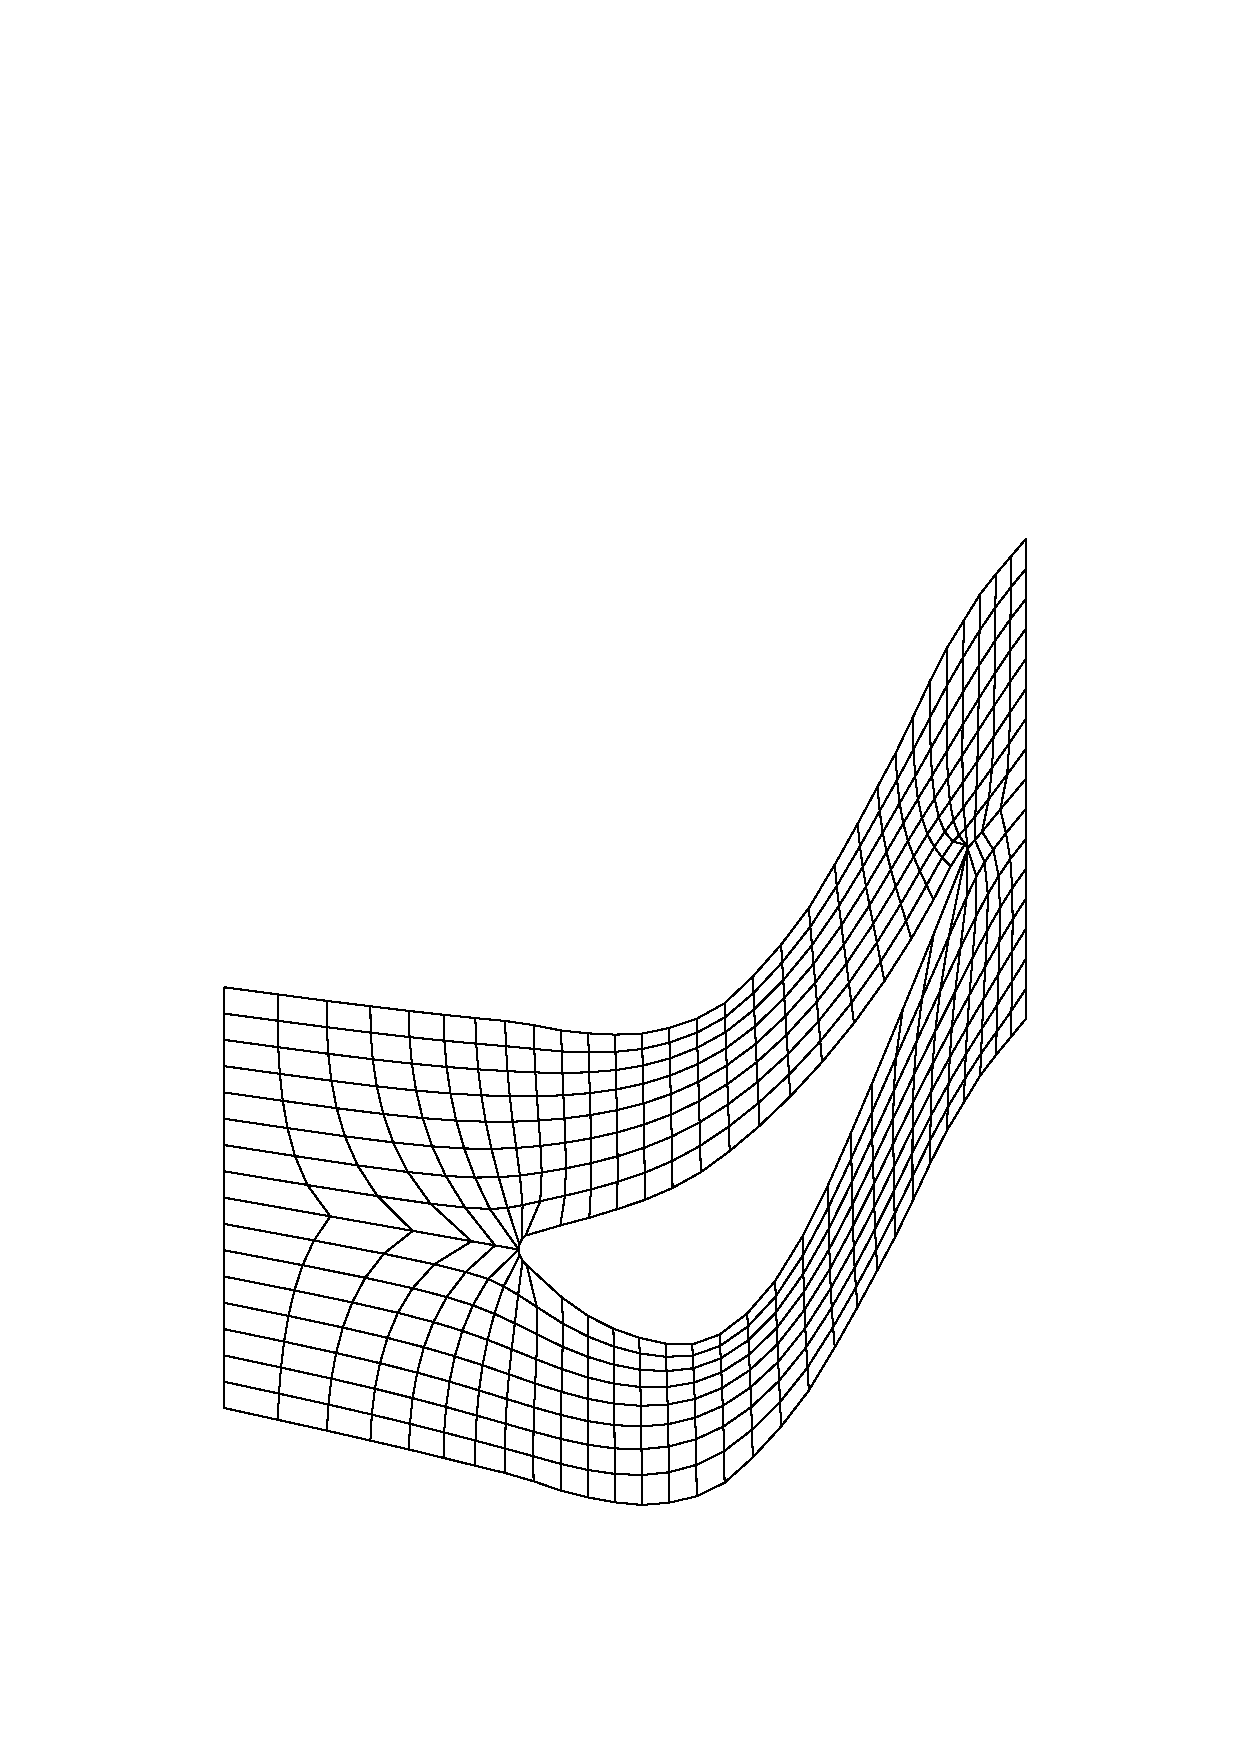
\includegraphics[width=45mm,clip=t]{CHAP_MESH/FIGURE/mesh2d_1_struct.pdf}\hspace{10mm}}
      &
      {\hspace{10mm}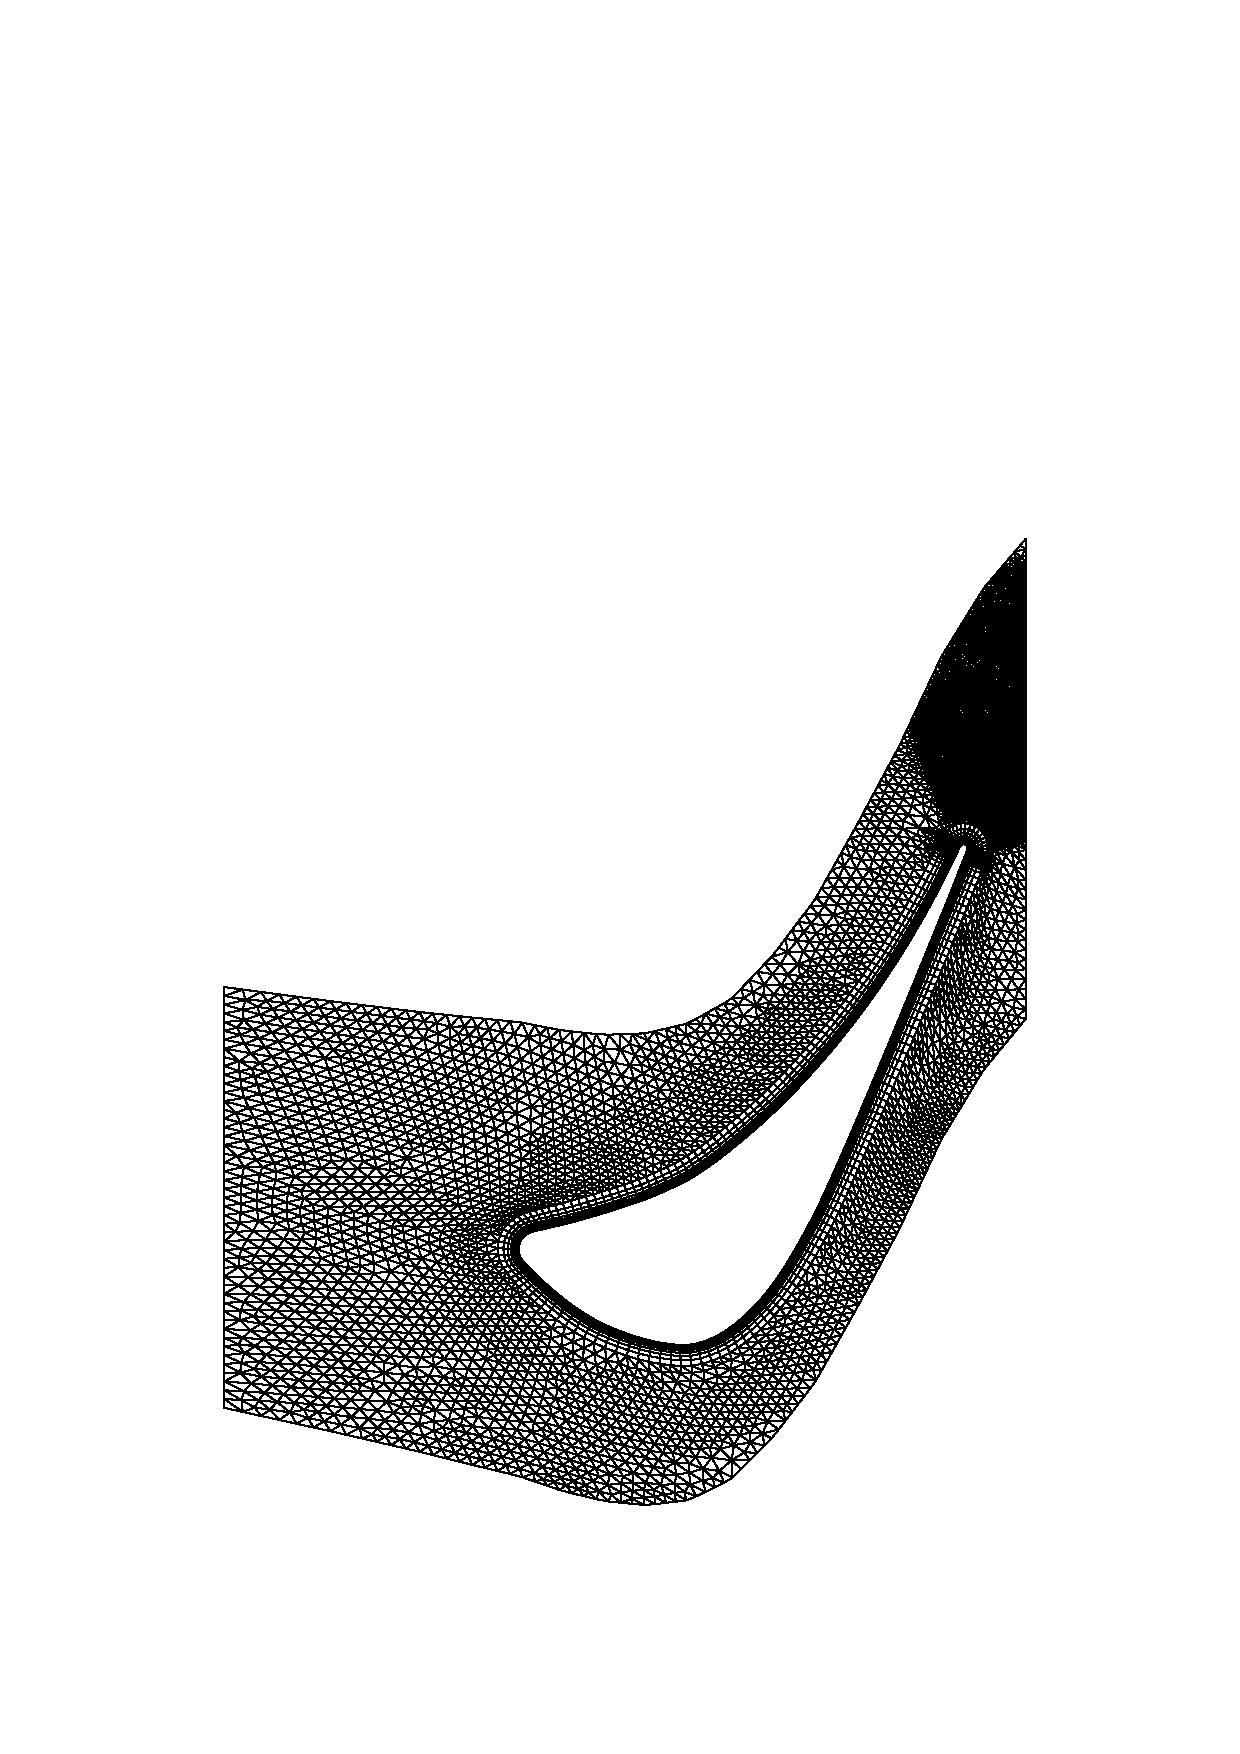
\includegraphics[width=45mm,clip=t]{CHAP_MESH/FIGURE/mesh2d_1_unstruct.pdf}}
      \end{tabular}}
    \\
    \subfigure[Middle section]
      {\begin{tabular}{cc}
      {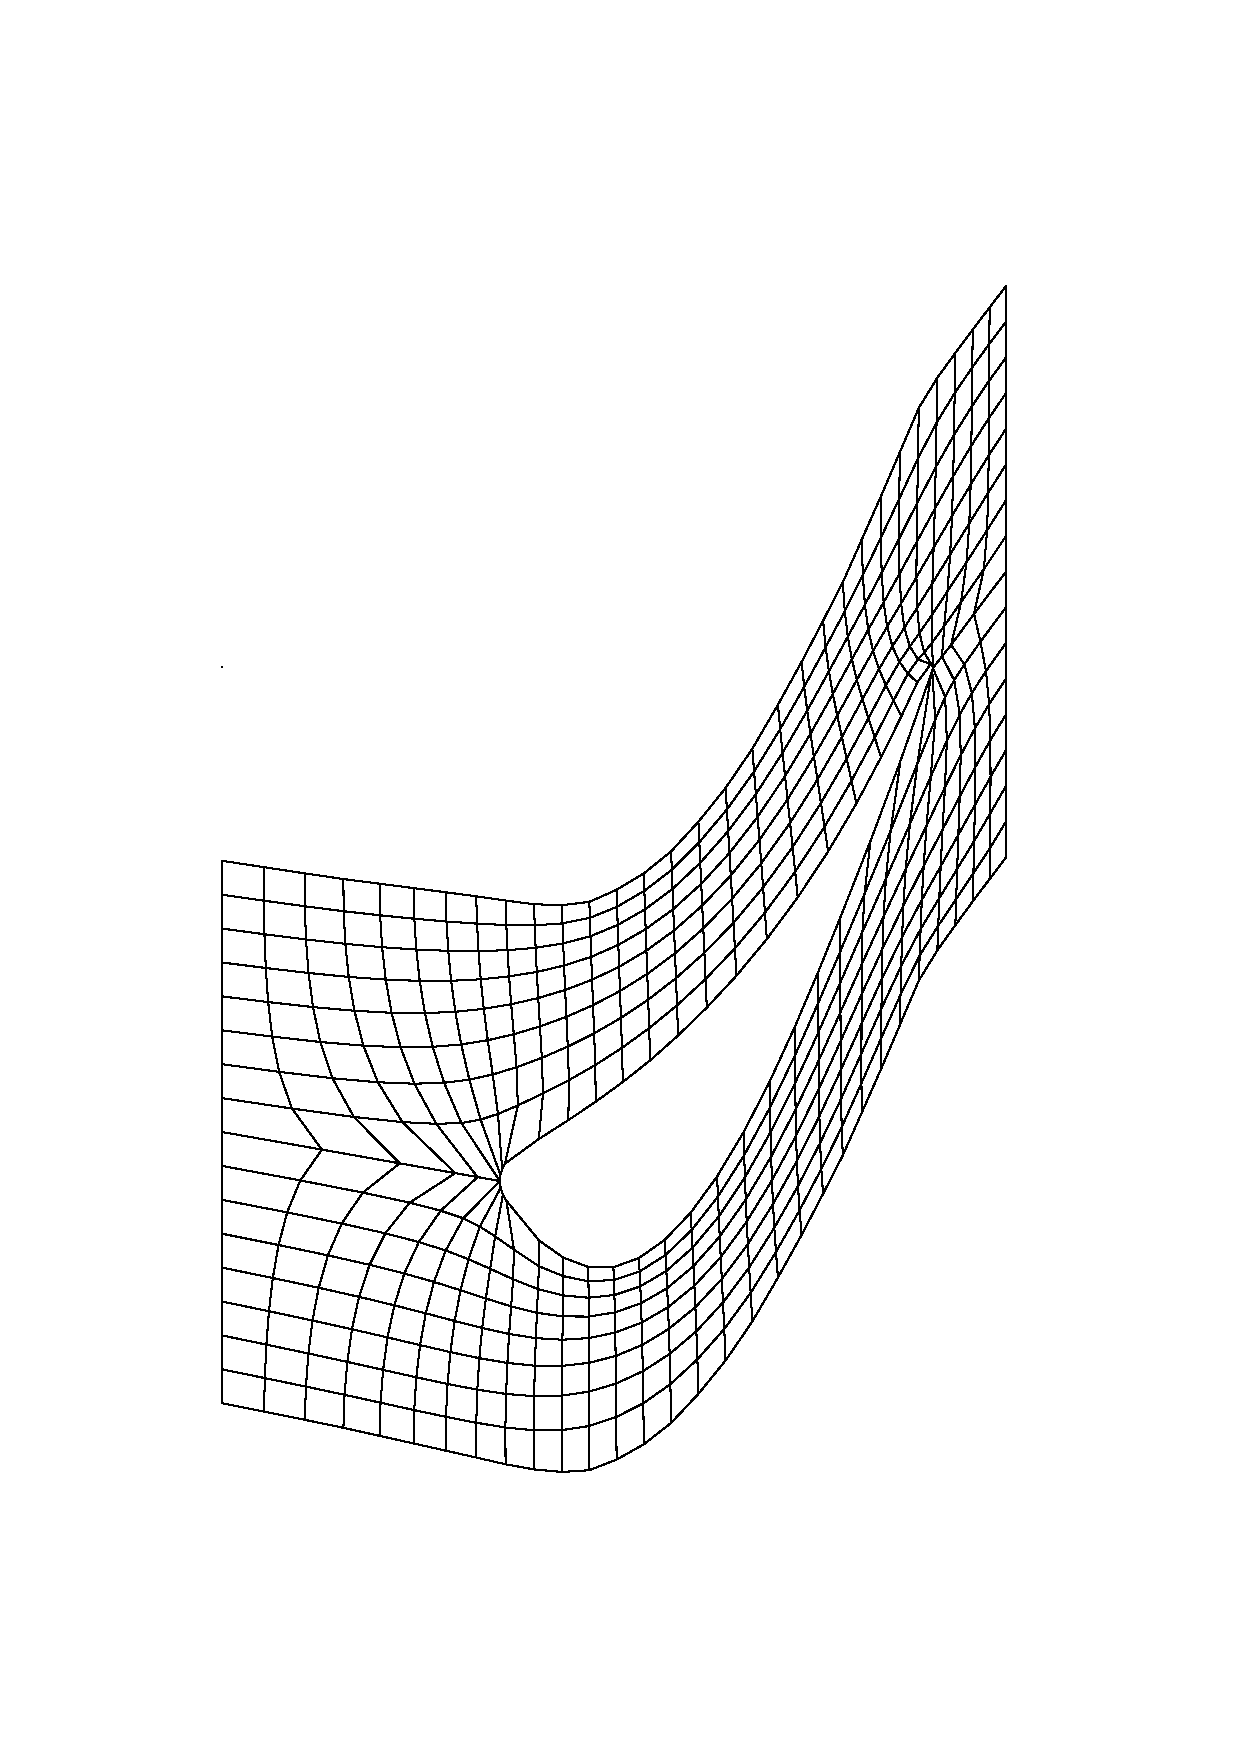
\includegraphics[width=45mm,clip=t]{CHAP_MESH/FIGURE/mesh2d_2_struct.pdf}\hspace{10mm}}
      &
      {\hspace{10mm}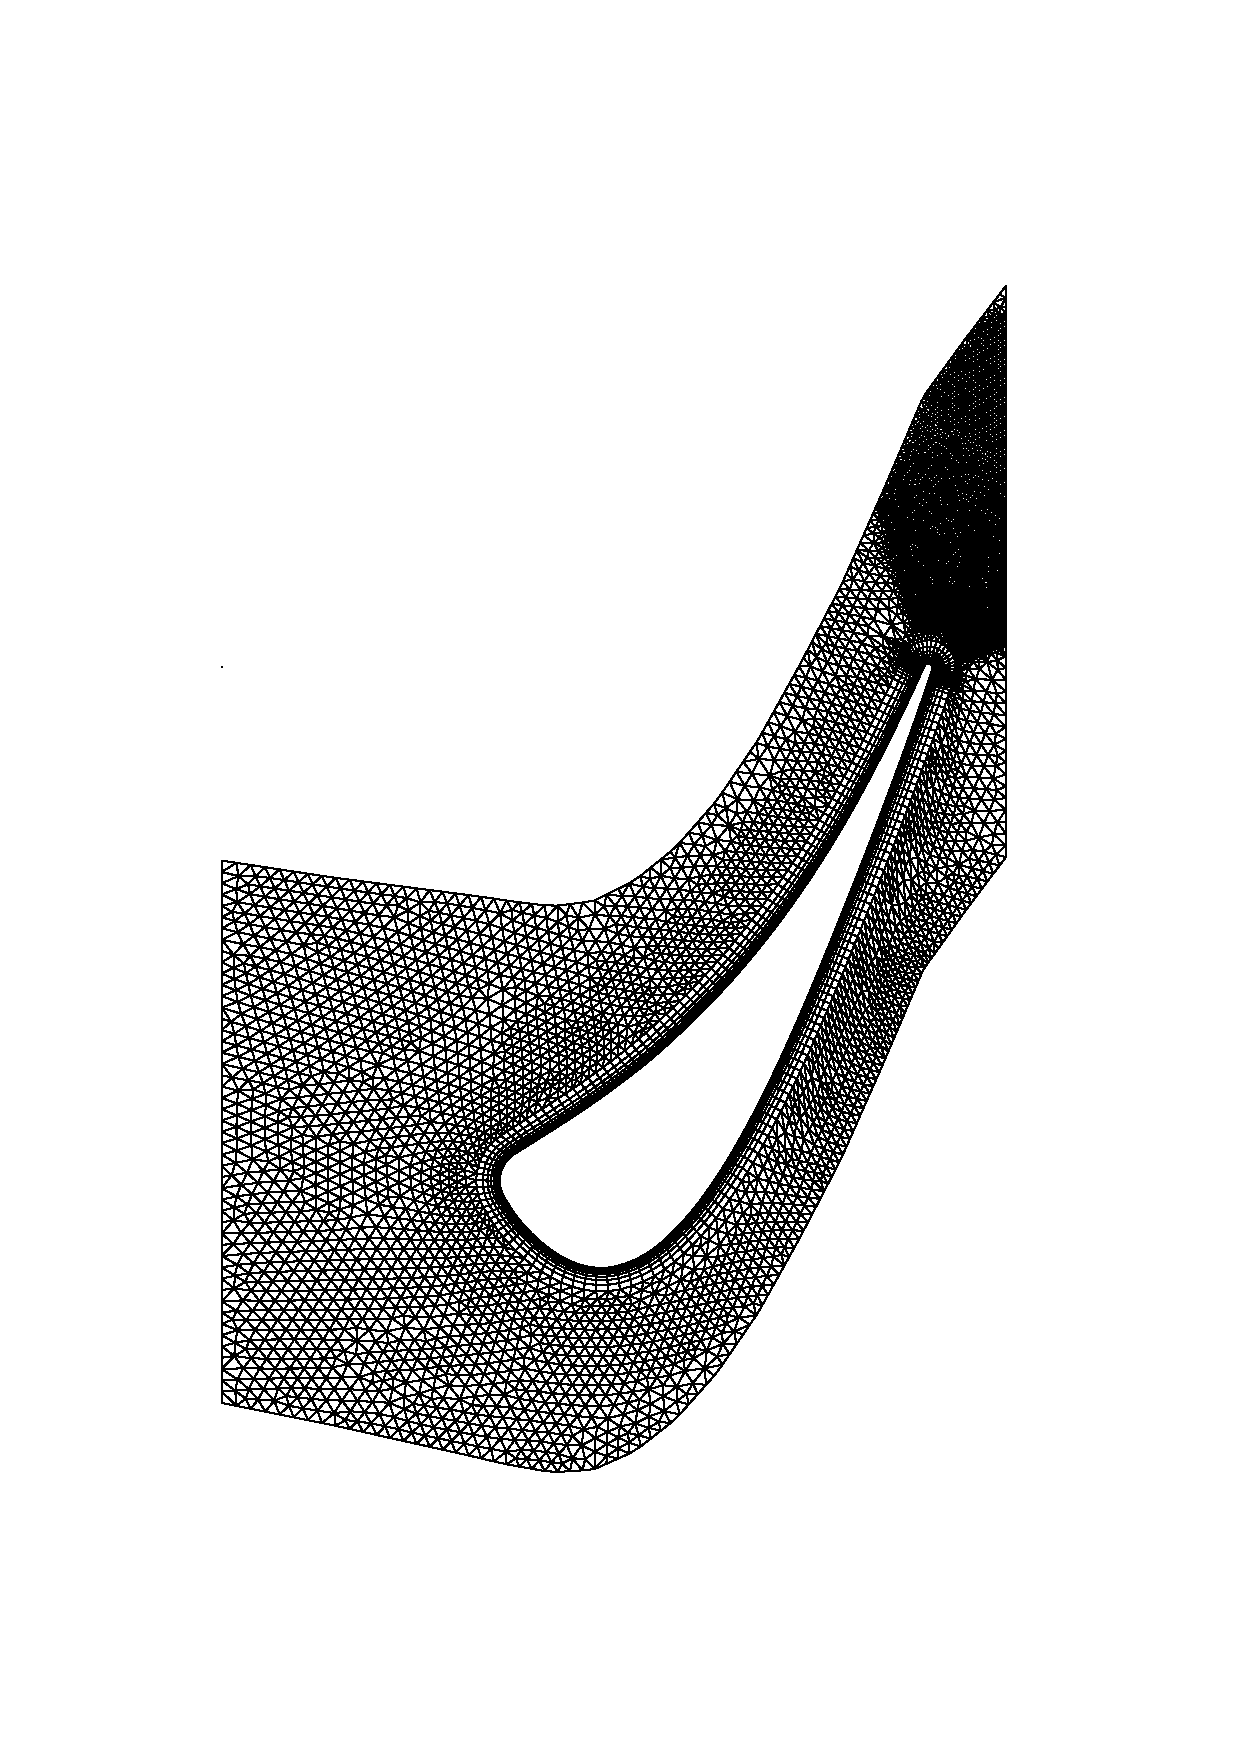
\includegraphics[width=45mm,clip=t]{CHAP_MESH/FIGURE/mesh2d_2_unstruct.pdf}}
      \end{tabular}}
    \\
    \subfigure[Tip section]
      {\begin{tabular}{cc}
      {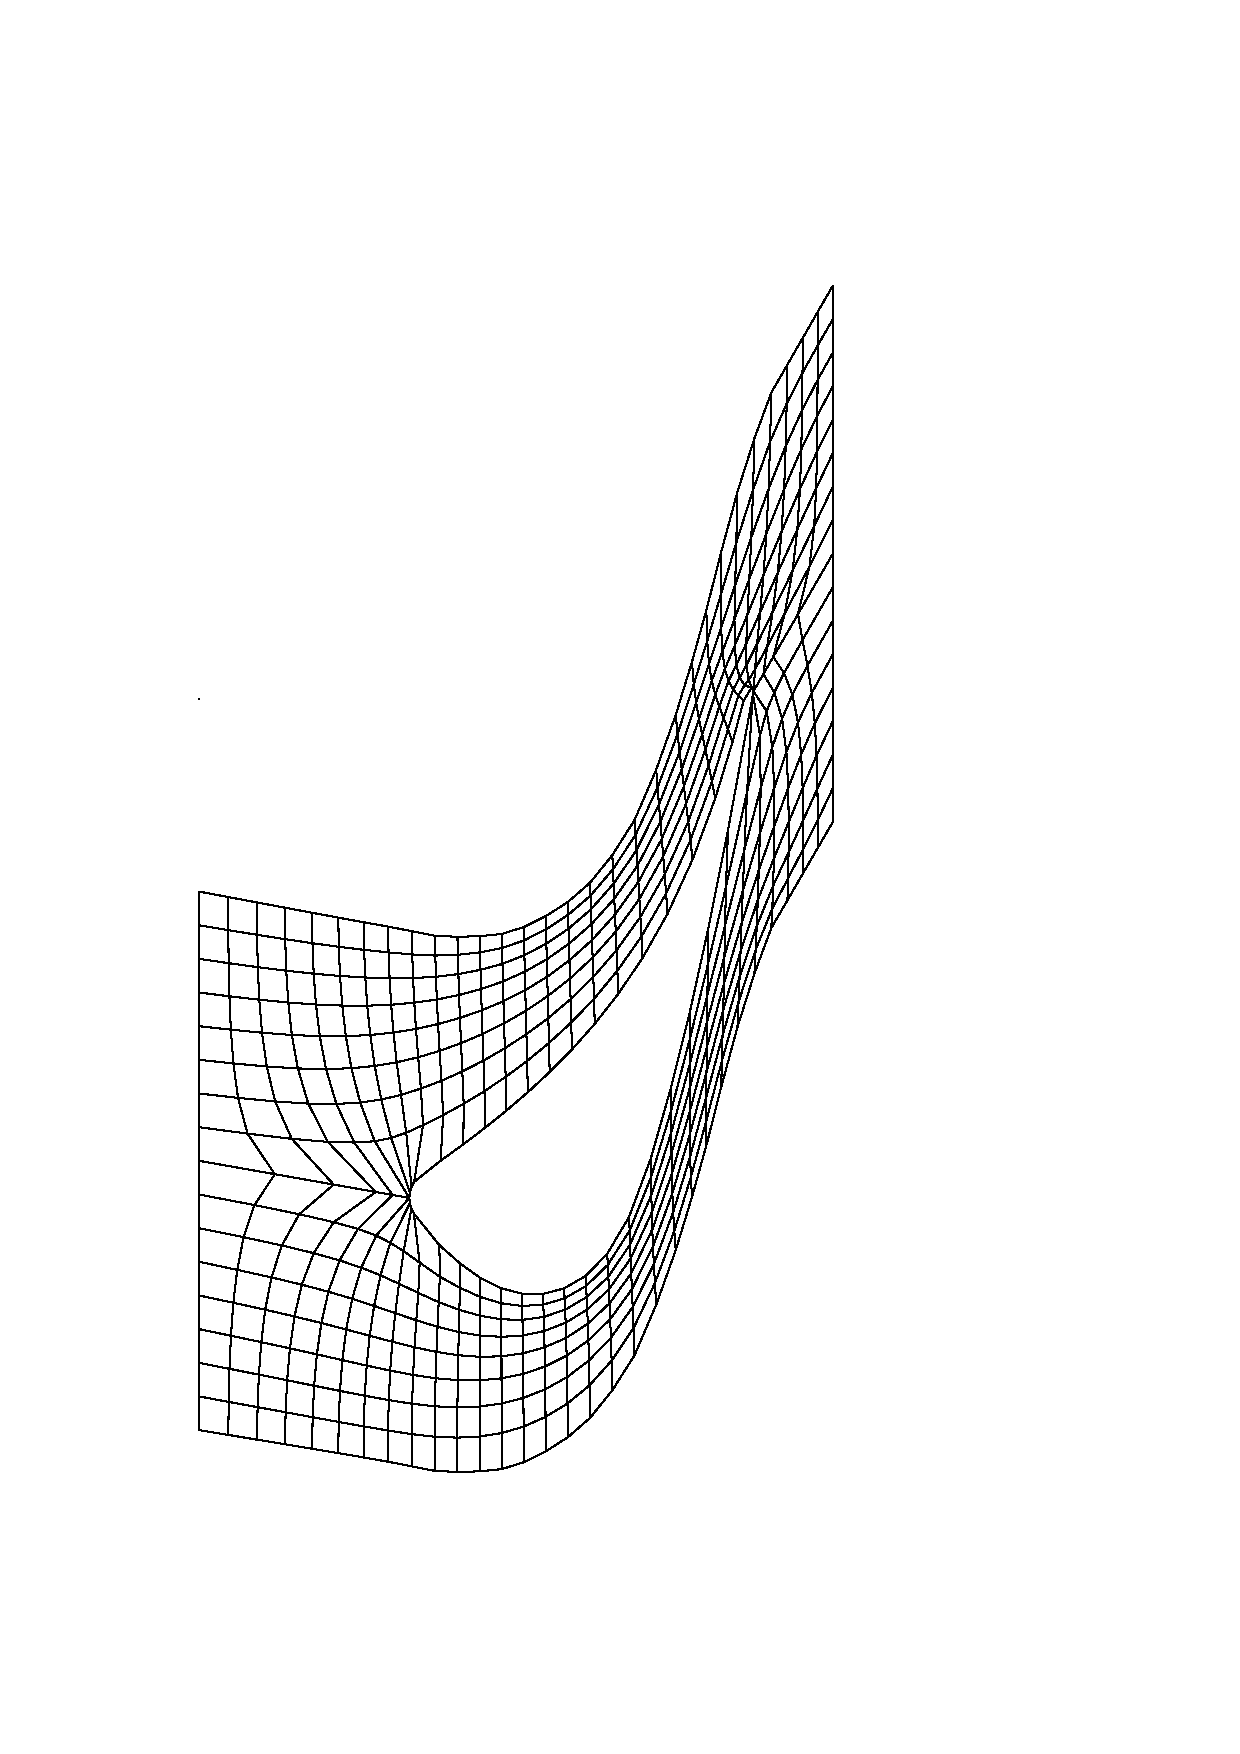
\includegraphics[width=45mm,clip=t]{CHAP_MESH/FIGURE/mesh2d_3_struct.pdf}\hspace{10mm}}
      &
      {\hspace{10mm}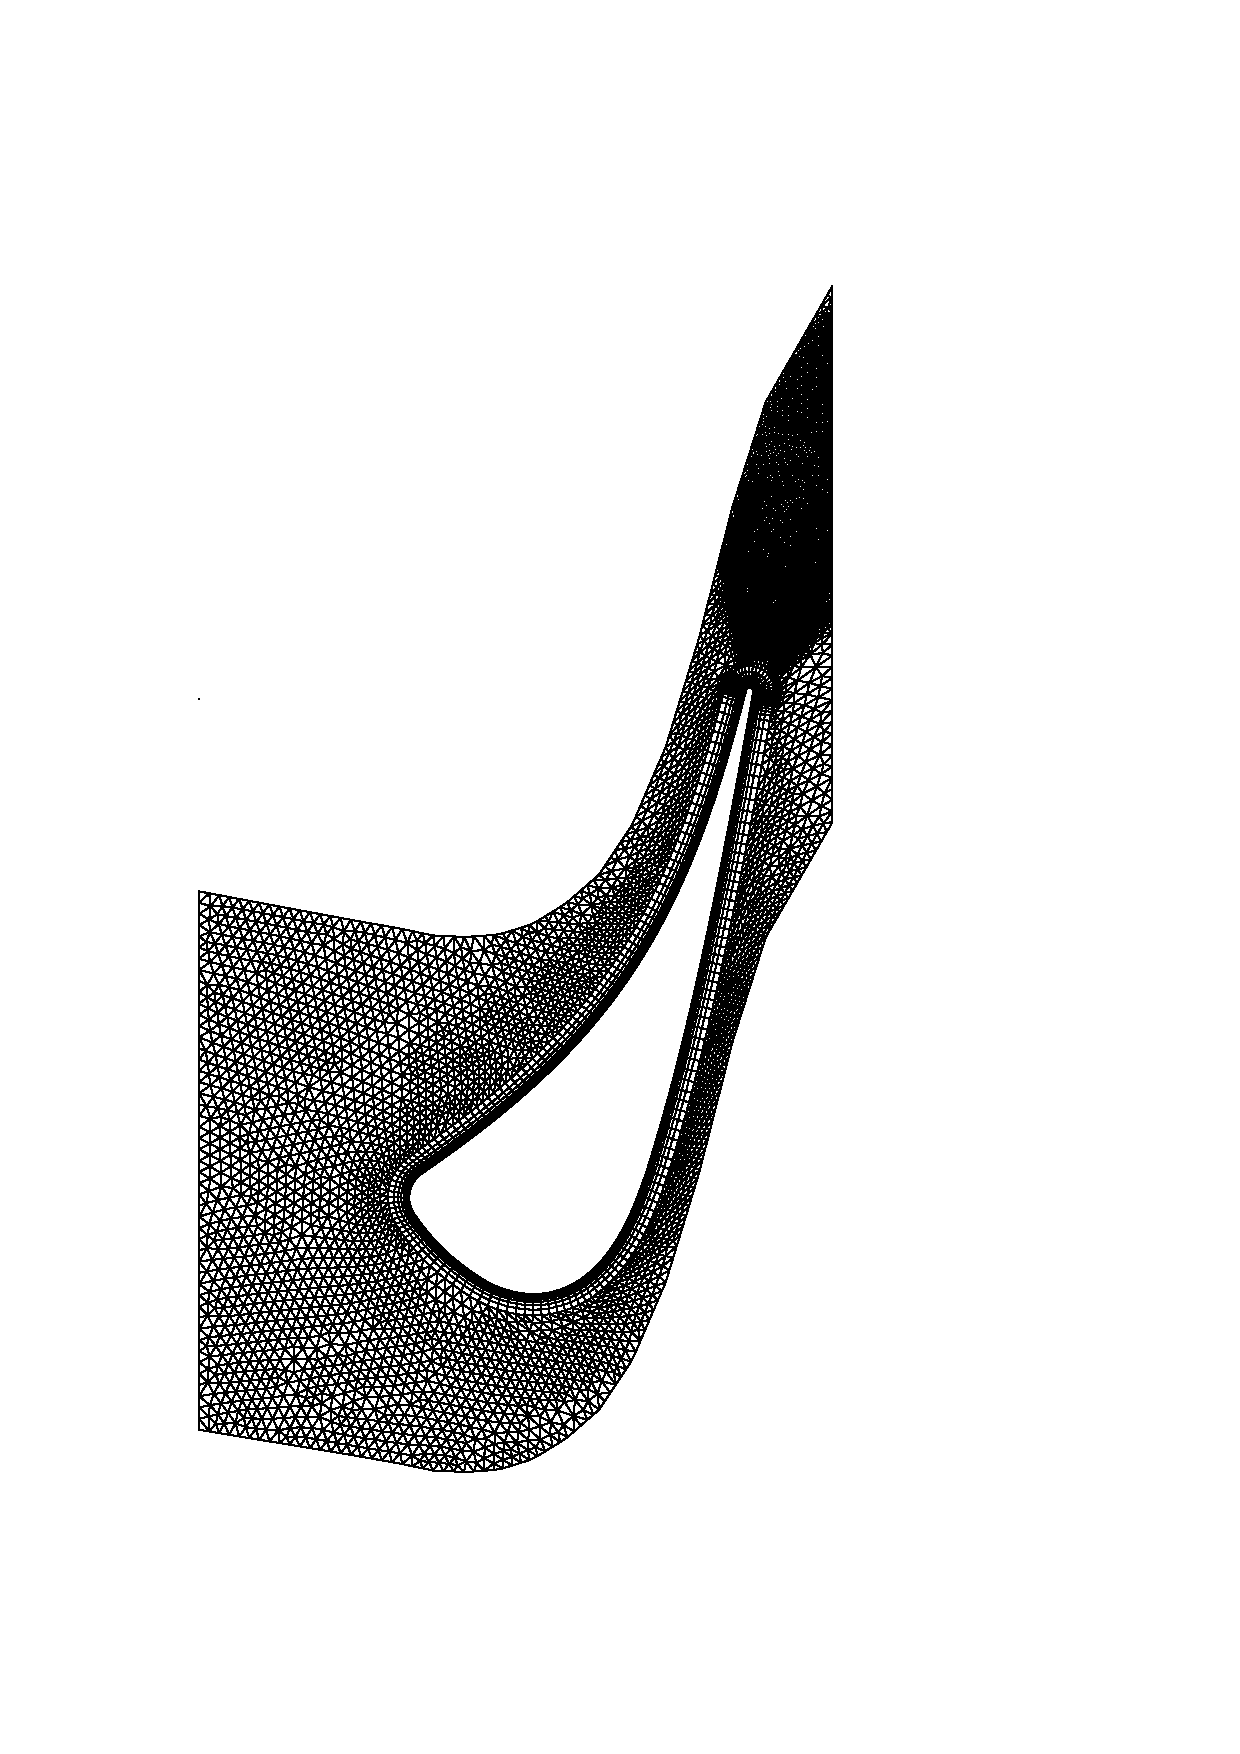
\includegraphics[width=45mm,clip=t]{CHAP_MESH/FIGURE/mesh2d_3_unstruct.pdf}}
      \end{tabular}}
  \end{tabular}
 \end{center}
 \vspace{-5mm}
 \caption{Structured meshes for mapping and corresponding mapped unstructured meshes at three radial levels}
 \label{mesh2d_other.fig}
\end{figure}
%
 Once the unstructured mesh has been mapped to all radial blade surfaces,
 a prismatic mesh is obtained by simply connecting the
 corresponding points at consecutive levels. Moreover,
 in order to enhance the quality of the 3D mesh, a
 smoothing procedure is performed. This operation
 alters the positions of the interior nodes without changing
 the topology of the mesh.
 The element sides are considered as springs of stiffness proportional
 to the length of the side. The nodes are moved until the spring system
 is in equilibrium, the position of which is found by Jacobi
 iterations.
%
%
%
\section{The Program LEVMAP}
\headb{Semi-structured Mesh Generator}{The program LEVMAP}
%
 The semi-structured mesh generation technique proposed in this Chapter
 has been implemented in the program LEVMAP (LEVel MAPping) written in
 Fortran 90. The LEVMAP program became a standard facility not only
 at the Vibration Centre but also at major aeroengine
 manifacturer. It is now used by
 many researchers and engineers for aerolasticity
 calculations on turbomachinery blades.
%
\begin{figure}[ht]
   \centerline{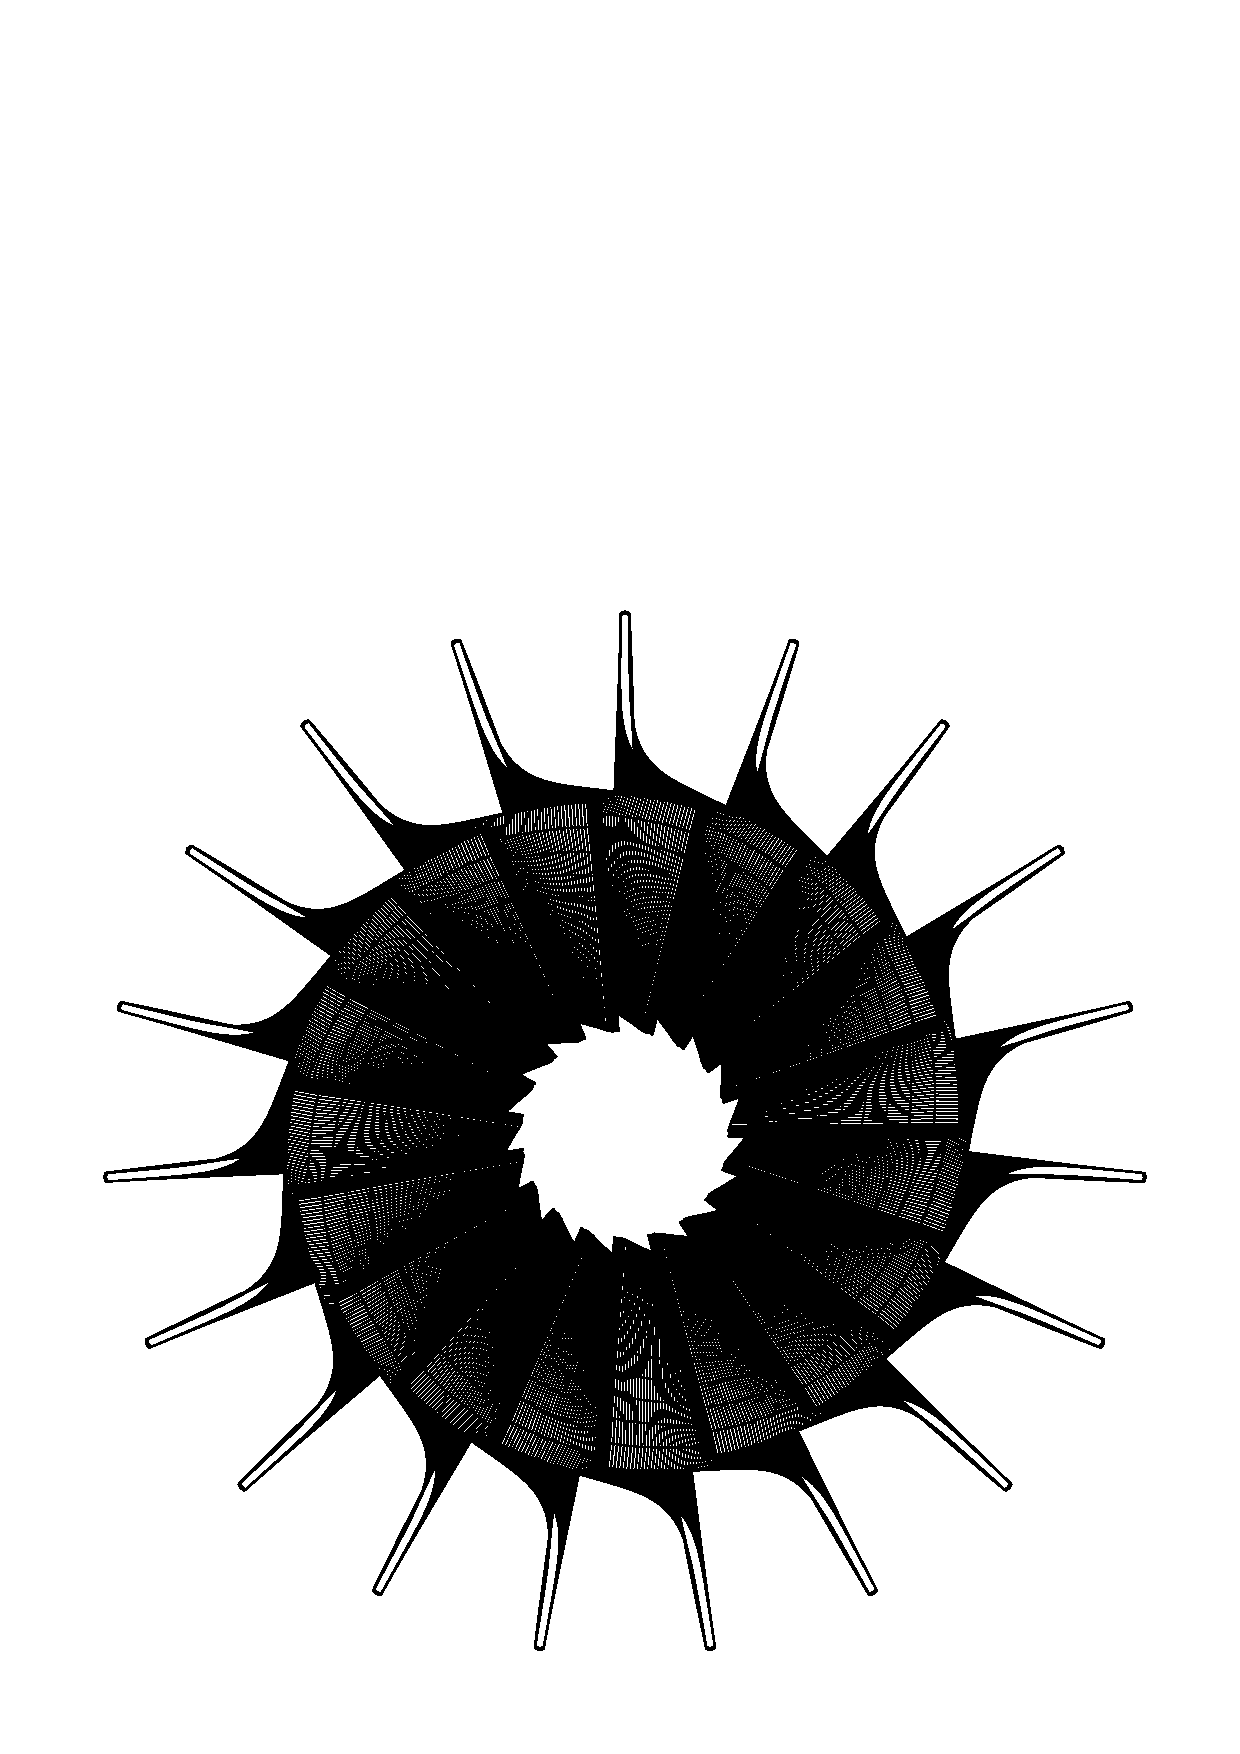
\includegraphics[width=140mm,clip=t]{CHAP_MESH/FIGURE/radial.pdf}}
   \caption{Semi-structured mesh for a radial-flow turbomachine}
   \label{radial_flow.fig}
\end{figure}
%
 A user's guide is available for the second release of the program
 (Sbardella \citeyearNP{Luca:5}).
 Grosclaude et al. \citeyear{Luca:8} extended LEVMAP to radial-flow
 turbomachine blades by modifying the 3D to 2D projection of
 Section \ref{geometry_modelling.sec}. An example of a semi-structured mesh
 for a radial turbomachinery assembly is shown in Fig. \ref{radial_flow.fig}.
 Further improvements of LEVMAP include automatic meshing of
 fan assembly + intake-duct, non-axisymmetric hub and tip, hub gap and
 snubber blades.
 Fig. \ref{snab_flow.fig} shows an exemple of semi-unstructured mesh for
 a snubbered fan blade assembly.
%
\begin{figure}[ht]
   \centerline{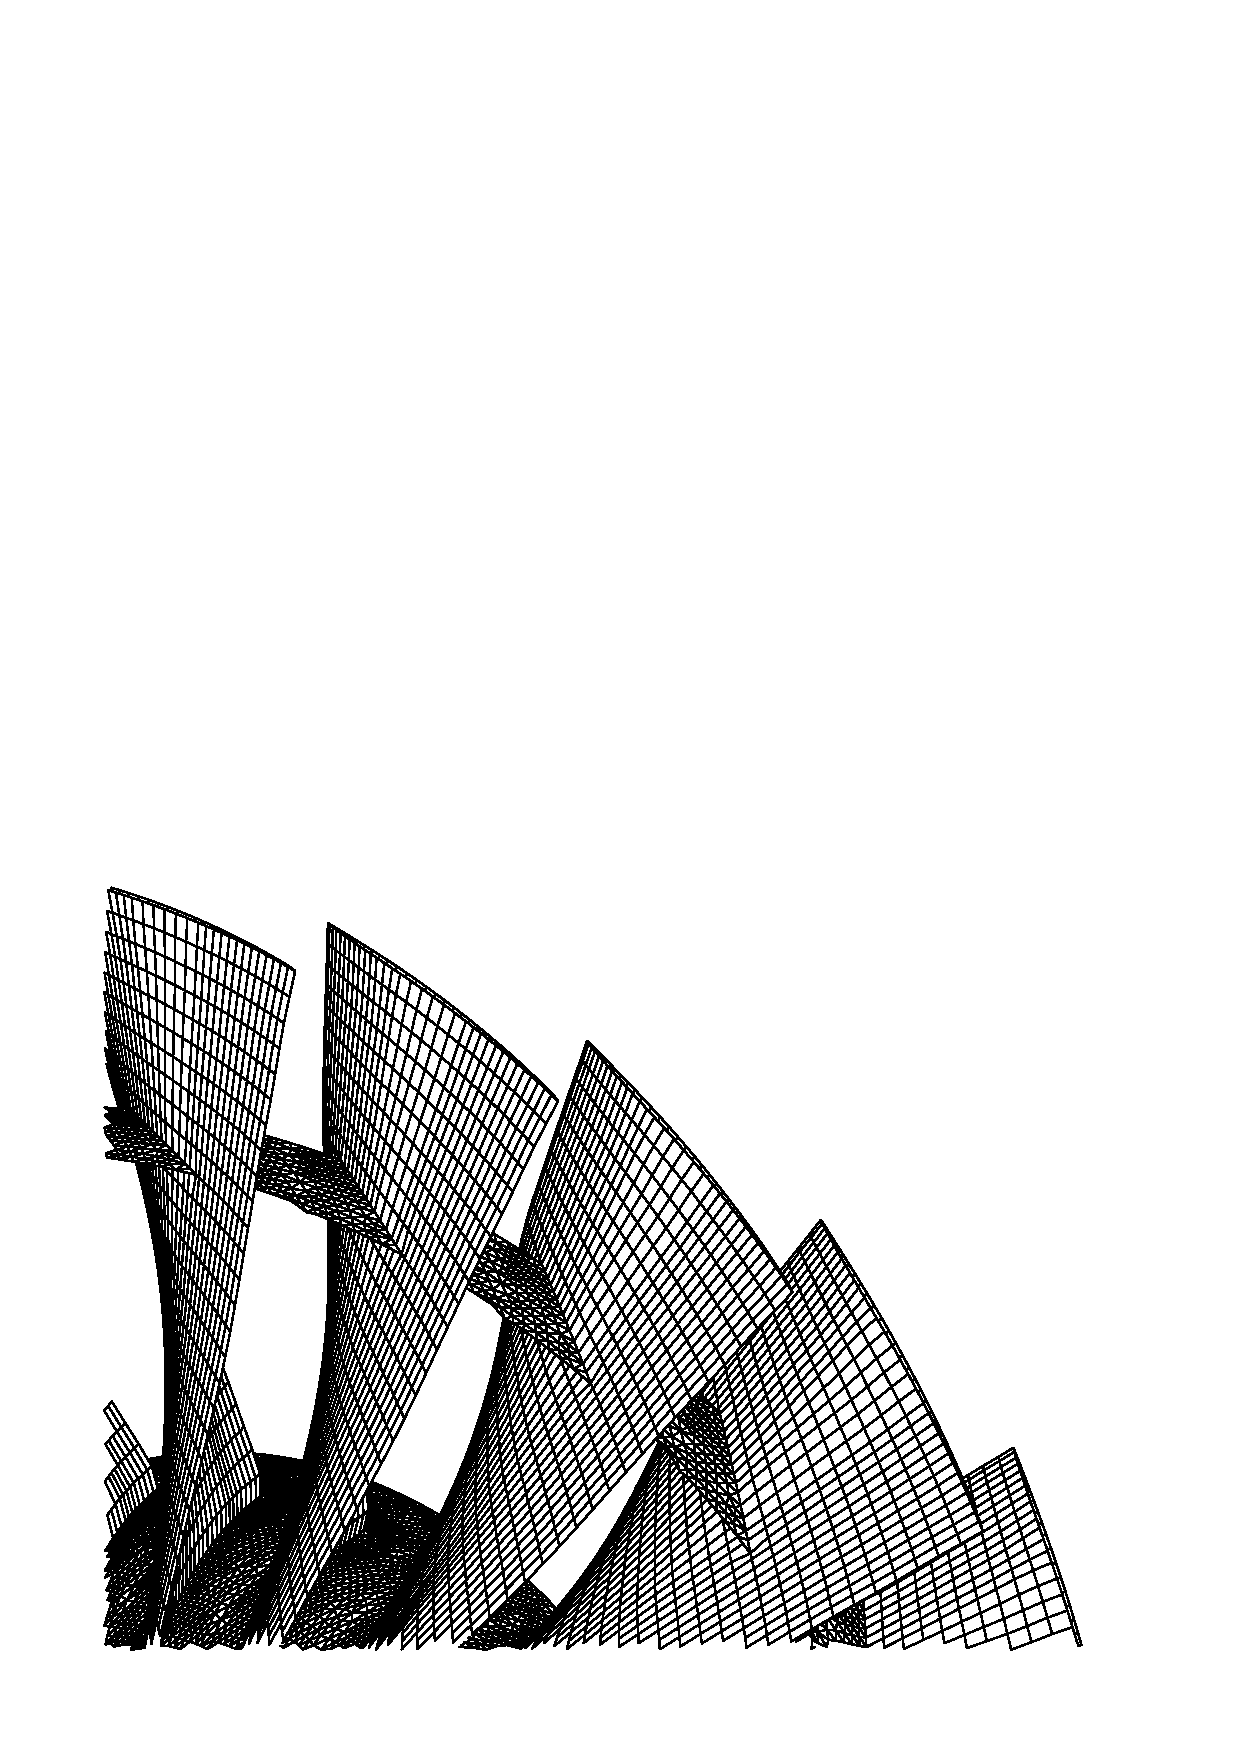
\includegraphics[width=120mm,clip=t]{CHAP_MESH/FIGURE/snab.pdf}}
   \caption{Semi-structured mesh for a snubbered fan assembly}
   \label{snab_flow.fig}
\end{figure}
%
%
%
%%%%%%%%%%%%%%%%%%%%%%%%%%%%%%%%%%%%%%%%%%%%
%%%%%%%      CONCLUDING REMARKS
%%%%%%%%%%%%%%%%%%%%%%%%%%%%%%%%%%%%%%%%%%%%
%
\section{Concluding Remarks}
\headb{Semi-structured Mesh Generator}{Concluding Remarks}
%
 A method to generate semi-structured prismatic meshes for turbomachinery
 blades has been presented. The unstructured mesh in the axial and
 tangential directions offers
 more flexibility than standard structured H-type, O-type and C-type meshes,
 both in terms of skewness minimization and smoothness optimization.
 The use of fully unstructured viscous meshes for blade like geometries
 is likely to require a much larger number of grid points and hence there
 are distinct advantages in using semi-structured meshes.
 Such was the success of the method that it was adopted by a major aeroengine
 manifacturer within one year of it being available.
